% Options for packages loaded elsewhere
\PassOptionsToPackage{unicode}{hyperref}
\PassOptionsToPackage{hyphens}{url}
%
\documentclass[
  12pt,
]{article}
\usepackage{amsmath,amssymb}
\usepackage{iftex}
\ifPDFTeX
  \usepackage[T1]{fontenc}
  \usepackage[utf8]{inputenc}
  \usepackage{textcomp} % provide euro and other symbols
\else % if luatex or xetex
  \usepackage{unicode-math} % this also loads fontspec
  \defaultfontfeatures{Scale=MatchLowercase}
  \defaultfontfeatures[\rmfamily]{Ligatures=TeX,Scale=1}
\fi
\usepackage{lmodern}
\ifPDFTeX\else
  % xetex/luatex font selection
  \setmainfont[]{Times New Roman}
\fi
% Use upquote if available, for straight quotes in verbatim environments
\IfFileExists{upquote.sty}{\usepackage{upquote}}{}
\IfFileExists{microtype.sty}{% use microtype if available
  \usepackage[]{microtype}
  \UseMicrotypeSet[protrusion]{basicmath} % disable protrusion for tt fonts
}{}
\makeatletter
\@ifundefined{KOMAClassName}{% if non-KOMA class
  \IfFileExists{parskip.sty}{%
    \usepackage{parskip}
  }{% else
    \setlength{\parindent}{0pt}
    \setlength{\parskip}{6pt plus 2pt minus 1pt}}
}{% if KOMA class
  \KOMAoptions{parskip=half}}
\makeatother
\usepackage{xcolor}
\usepackage[margin=1in]{geometry}
\usepackage{graphicx}
\makeatletter
\def\maxwidth{\ifdim\Gin@nat@width>\linewidth\linewidth\else\Gin@nat@width\fi}
\def\maxheight{\ifdim\Gin@nat@height>\textheight\textheight\else\Gin@nat@height\fi}
\makeatother
% Scale images if necessary, so that they will not overflow the page
% margins by default, and it is still possible to overwrite the defaults
% using explicit options in \includegraphics[width, height, ...]{}
\setkeys{Gin}{width=\maxwidth,height=\maxheight,keepaspectratio}
% Set default figure placement to htbp
\makeatletter
\def\fps@figure{htbp}
\makeatother
\setlength{\emergencystretch}{3em} % prevent overfull lines
\providecommand{\tightlist}{%
  \setlength{\itemsep}{0pt}\setlength{\parskip}{0pt}}
\setcounter{secnumdepth}{-\maxdimen} % remove section numbering
\newlength{\cslhangindent}
\setlength{\cslhangindent}{1.5em}
\newlength{\csllabelwidth}
\setlength{\csllabelwidth}{3em}
\newlength{\cslentryspacingunit} % times entry-spacing
\setlength{\cslentryspacingunit}{\parskip}
\newenvironment{CSLReferences}[2] % #1 hanging-ident, #2 entry spacing
 {% don't indent paragraphs
  \setlength{\parindent}{0pt}
  % turn on hanging indent if param 1 is 1
  \ifodd #1
  \let\oldpar\par
  \def\par{\hangindent=\cslhangindent\oldpar}
  \fi
  % set entry spacing
  \setlength{\parskip}{#2\cslentryspacingunit}
 }%
 {}
\usepackage{calc}
\newcommand{\CSLBlock}[1]{#1\hfill\break}
\newcommand{\CSLLeftMargin}[1]{\parbox[t]{\csllabelwidth}{#1}}
\newcommand{\CSLRightInline}[1]{\parbox[t]{\linewidth - \csllabelwidth}{#1}\break}
\newcommand{\CSLIndent}[1]{\hspace{\cslhangindent}#1}
\usepackage{setspace}\doublespacing
\usepackage{booktabs}
\usepackage{longtable}
\usepackage{array}
\usepackage{multirow}
\usepackage{wrapfig}
\usepackage{float}
\usepackage{colortbl}
\usepackage{pdflscape}
\usepackage{tabu}
\usepackage{threeparttable}
\usepackage{threeparttablex}
\usepackage[normalem]{ulem}
\usepackage{makecell}
\usepackage{xcolor}
\ifLuaTeX
  \usepackage{selnolig}  % disable illegal ligatures
\fi
\IfFileExists{bookmark.sty}{\usepackage{bookmark}}{\usepackage{hyperref}}
\IfFileExists{xurl.sty}{\usepackage{xurl}}{} % add URL line breaks if available
\urlstyle{same}
\hypersetup{
  pdftitle={Quantifying Stability and Change in Personal Culture Using Panel Data},
  hidelinks,
  pdfcreator={LaTeX via pandoc}}

\title{Quantifying Stability and Change in Personal Culture Using Panel
Data}
\author{}
\date{\vspace{-2.5em}}

\begin{document}
\maketitle
\begin{abstract}
Recent work has produced conflicting interpretations on the question of
whether adults undergo durable changes in their personal culture over
time. This paper asserts that this divergence is less due to
researchers' findings than the approach taken -- a tournament of models
focusing on the presence or absence of change. To move beyond this, we
reanalyze the data used previously in this debate with an approach that
quantifies the processes of cultural difference. In doing so, we compare
how much cultural difference is explained by intrapersonal change and
interpersonal differences. Our results harmonize recent findings by
showing that, while most measures of personal culture show change over
time, the variance explained by intrapersonal change is typically small
compared to interpersonal differences at baseline. Quantifying these
processes offers new ways to address theoretical questions of when and
how their relative importance shifts. We examplify this approach by
exploring how the importance of these processes differs between college
graduates and the rest of the population.
\end{abstract}

\hypertarget{introduction}{%
\section{Introduction}\label{introduction}}

Does personal culture---an individual's attitudes, beliefs, values, and
practices---change over the life course, or is it largely fixed by
adulthood? This question underlies an important contemporary debate in
sociology (Kiley and Vaisey 2020; Lersch 2023; Lizardo 2017) and has
deep roots in seemingly contradictory theoretical perspectives. For
example, pragmatist theories of action claim that changes in social
environments cause people to adapt their views and make new cultural
meanings (Gross 2009; Swidler 2001), while Bourdieusian practice
theories argue that the ``past conditions of production'' leave a mark
on people's personal culture that lasts throughout their lives (Bourdieu
1990). Models of social influence assume that people adapt their culture
in the face of new information (Goldberg and Stein 2018), while the
emphasis on cohort effects in models of aggregate social and cultural
change requires them to be open to change while young but become fairly
resistant to it as they age (Ryder 1965). Finally, life course theories
posit important changes over time as people advance through important
transitions in their lives (Bardi et al. 2009; Elder, Johnson, and
Crosnoe 2003).

Because all of these theoretical perspectives have some empirical
support, the current debate is not about whether their posited processes
exist at all, but about their relative contribution to explaining the
cultural differences we see in the world. That said, scholars have
struggled to reach a consensus on the importance of change during
adulthood. Over the span of a few years, most apparent changes in
people's responses to personal survey items appear to be transitory,
with little evidence of persistent change among adults (Kiley and Vaisey
2020; Vaisey and Kiley 2021). This suggests that change during adulthood
is not a major factor in explaining personal cultural differences. When
we consider a longer time horizon, however, there is evidence that
adults make at least some persistent changes (Lersch 2023).

These seemingly inconsistent findings are partly due to the fact that
researchers have taken a ``tournament of models'' approach to
adjudicating different theoretical perspectives (Lersch 2023: p.~228).
That is, researchers have compared the fit of different statistical
models to each item to determine whether it is more consistent with ``no
change'' or ``any change.'' The size of these piles then serves as the
primary evidence for the truth of the theory (Kiley and Vaisey 2020;
Lersch 2023; Vaisey and Kiley 2021).

We argue, however, that asking \emph{whether} people change on an item
may cause more problems than it solves. Being able to detect \emph{any}
change on an item depends not only on sample populations, measurement,
statistical methods, and power, but also on definitions of what counts
as ``change.'' These differences can limit the possibility of agreement
on which ``pile'' a variable belongs in. Moreover, asking whether there
is evidence of change reduces to, ``Is there \emph{any} evidence of
change in this item?'' But such binary inquiries are ill-suited to
address the core of the theoretical debate: determining \emph{how much}
the process of intrapersonal change contributes to cultural differences.

There is enough evidence to assert that neither pre-adult socialization
nor the contemporary social context alone can explain the full range of
cultural differences. The question that remains is about the
\emph{relative} contributions of these processes. In the current debate,
for a single construct (e.g., support for gay rights), existing
approaches can only make claims about \emph{whether} intrapersonal
change is happening, not about how much. This also prevents
investigating under what conditions, across which groups, and in what
domains do we see differences in the relative importance of
intrapersonal change and pre-existing interpersonal differences. These
questions are about \emph{degree}, not existence; taking this debate
forward will require precise measurement rather than declarations of
victory for a particular perspective.

In this paper, we move beyond the ``tournament of models'' approach and
introduce a method for quantifying the relative contributions of
interpersonal differences and intrapersonal change for a single item.
Drawing on seven panel data sets from five countries, we quantify the
amount of variance in survey responses that is due to between-person
differences at a single point during the survey versus the amount of
variance in responses that is due to systematic intrapersonal change
over the study period. This measure quantifies the amount of change over
the duration of the panel relative to the stable differences that exist
between people.

Using this measure, we observe similar patterns across the datasets that
have previously yielded conflicting interpretations. In all
datasets---despite their varied social contexts and duration---we find a
similar distribution of intrapersonal change. In general, we find that
intrapersonal change accounts for a substantially smaller amount of
variance in personal culture survey item than stable interpersonal
differences. Of course, whether the amount of intrapersonal change in an
item is large enough to be ``meaningful'' is a substantive and
theoretical question. Nevertheless, on many measures of personal culture
(some observed for over a decade), we do not observe enough
intrapersonal change for it to play a substantial role in explaining the
differences we observe between adults. Notable, interesting, and
important exceptions exist, of course, but they are departures from the
overall pattern.

Our method can also help address substantive questions about personal
change. To illustrate this, we investigate differences in the relative
importance of intrapersonal change on political items for people with
and without a college degree. We find that change is less pronounced for
college-educated respondents, suggesting that college solidifies
political dispositions rather than fostering an openness to new
information. This offers a novel empirical basis to theorize about the
role of college in shaping personal culture . In summary, we believe
that this approach has the potential to advance the theoretical debate
on the role of environments, social identities, and roles in
facilitating personal cultural change and stability.

Taken together, to goal of this paper is to advance---and, hopefully,
transcend---debates about \emph{whether} adults change. They do change,
at least a little, on most things. Our method can help quantify exactly
how much.

\hypertarget{background}{%
\section{Background}\label{background}}

\hypertarget{change-and-stability-in-personal-culture}{%
\subsection{Change and Stability in Personal
Culture}\label{change-and-stability-in-personal-culture}}

Recent debates about whether adults undergo intrapersonal cultural
change emerged in part because theories of cultural change at the
aggregate level tend to implicitly invoke one of two models of
individual behavior. The first, what Kiley and Vaisey (2020) call a
``Settled Dispositions Model'' (SDM), assumes that peoples' personal
culture is relatively fixed by the time they are adults. While they
might make temporary changes in their declarative culture in reaction to
their environments, this model assumes that people return to a settled
baseline over a short period of time. This model underlies theories of
cultural change that suggest people are imprinted by early socialization
experiences such as the ``past conditions of production'' a Bourdieusian
practice theory (Bourdieu 1990), cohort replacement theories of
aggregate change (Mannheim 1952; Ryder 1965), and control theories in
social psychology (Robinson 2007; Smith-Lovin and Heise 1988).

The second model summarized by Kiley and Vaisey (2020), an ``Active
Updating Model'' (AUM), posits that people continually update their
personal culture as they move through life. This model suggests people
change their personal culture as they adapt and make new meanings when
encountering new social environments, discourses, and information (Gross
2009; Swidler 2001). This model underlies, among others, theories of
cultural diffusion (Christakis and Fowler 2010), attitude alignment
(DellaPosta 2020), and polarization (Bail et al. 2018). It is also
implicit in most studies that ask whether specific experiences, changes
in social roles, or political events, affect personal culture (Gelman
and Margalit 2021; Slothuus and Bisgaard 2021; Visser and Mirabile
2004).

There is no reason to believe that only one of these two models is
``correct'' at all times and in all places. A population observed over
some period of time contains a mix of people who are noticeably changing
and people who are not. Instead, different perspectives argue that each
of these ideal-typical models is more operative at different times, for
different people, and for different elements of personal culture. For
example, adolescence and early adulthood is typically viewed as a
``formative period'' for personal cultural development and thus
characterized by higher rates of active updating, while middle age and
later life are potentially characterized more by settled dispositions
(Alwin and Krosnick 1991; Eaton et al. 2009; Krosnick and Alwin 1989).
Similarly, salient issues, such as views around gay rights in the 2010s;
issues that see substantial elite realignments, such as views around the
Vietnam conflict in the 1970s (Zaller 1992); and novel issues of public
opinion, such as views around vaccines during the Covid-19 pandemic
(Scoville et al. 2022), might be characterized by active updating, while
established issues of low salience are characterized by stability.

Empirically comparing which of these models better fit a broad range of
questions from the General Social Survey's rotating panels, Kiley and
Vaisey (2020) found limited evidence of durable change. While the
majority of items preferred the AUM, the amount of durable change
detected on these items was small. A substantial minority of questions
(39 percent) favored the SDM, meaning they showed no evidence of durable
change. Questions with more evidence of durable change included salient
issues like gay marriage and questions tapping ``public'' statements or
behaviors such as partisan identification and religious service
attendance. There was also more evidence of durable change among early
adults (people ages 18-30) than the rest of the population. Overall, the
researchers concluded that ``results ultimately suggest that real,
persistent attitude change is an uncommon phenomenon among adults'\,'
(Kiley and Vaisey 2020: p.~500; see also Vaisey and Kiley 2021). This
lack of durable change is consistent with other recent findings that
cohort replacement plays a larger role than period effects in explaining
differences in personal culture (Vaisey and Lizardo 2016).

On the other hand, the claim that change is a relatively infrequent
phenomenon has been difficult to square with research identifying
durable change as a result of social experiences across a number of
cultural dimensions, such as morality (Broćić and Miles 2021), trust
(Mewes et al. 2021), and concerns about immigration (Kratz 2021).
Similarly, there are longitudinal studies showing that cues from
political elites can change an individual's position on specific policy
issues (Slothuus and Bisgaard 2021; Zaller 1992) and that changes in
their close contacts and acquaintances can change individuals' attitudes
on group-related politics (DellaPosta 2018; Gelman and Margalit 2021).
Given how often we observe people change their personal culture, it is
hard to accept that adults do not change.

Drawing on these findings, Lersch (2023) challenged the SDM and AUM as a
``needless dichotomy,'' proposing the ``Life Course Adaption Model''
(LCAM) as an alternative. This model draws on the life course
perspective to model personal culture as a different linear trajectory
over the duration of a panel for each respondent. In doing this, Lersch
rectified two shortcomings of the AUM and SDM. First, the AUM, as
described by Kiley and Vaisey, posits that changes follow a Markov
process where responses at time \(t\) are a function of responses at
time \(t-1\) but not earlier time points. However, earlier life
experiences can (directly and indirectly) mold personal culture when
transitioning to new social roles or into new environments, even if
their initial impact is delayed. For example, childhood events might
influence views on family structures later when individuals form their
own families. Therefore, the LCAM considers influences from earlier than
just \(t-1\) on responses at time \(t\).

Second, Kiley and Vaisey's analysis of the AUM and SDM is based on
three-wave panel data over four years, which might not be extensive
enough to adjudicate the two models. Lersch evaluates the LCAM against
the AUM and SDM using panel data spanning a wider duration (from 3 to 36
years) and more waves (3 to 18), offering a better chance to observe
durable change.

When Lersch compared the LCAM to the AUM and SDM on data from five
countries, 297 of the 428 questions he analyzed preferred the LCAM,
suggesting that we observe some linear change for adults on most items.
The SDM was preferred on 112 items, and the rest did not yield
conclusive results. No questions favored the AUM. He concludes that
``new experiences over the life course {[}\ldots{]} can persistently
move individuals' personal culture in novel directions'' (Lersch 2023:
p.~243-244).

Despite differences in how these researchers interpret their findings,
the empirical results are not far apart. Kiley and Vaisey (2020) found
that the majority of items they tested favored the AUM, meaning there
was evidence of durable change among adults, a pattern consistent with
Lersch's results. While Lersch (2023) found evidence of durable change
on most items, this change only accounted for a small proportion of
variance explained. On average, people changed only about .07 standard
deviations over 10 years. This is consistent with Kiley and Vaisey's
finding that durable change is often small. And a quarter of the items
Lersch studied still preferred the SDM, suggesting that even with
different assumptions assumptions about change and more extensive data,
many questions show no evidence of durable change. Likewise, in studies
showing evidence of durable change in specific measures of personal
culture, the change is often small. For example, Brocic and Miles (2021)
estimate that completing graduate degrees in humanities, arts, and
social sciences shift peoples' moral relativism only about .2 standard
deviations on average compared to people with no college degree, and
this is the largest effect they identify. And studies of aggregate
change show that, even on items where cohort effects explain more
variance than period effects, there is always evidence that some people
change over time (Vaisey and Lizardo 2016). In other words, despite
different interpretations, the results of previous work are in many ways
highly consonant.

\hypertarget{quantification-not-adjudication}{%
\subsection{Quantification, Not
Adjudication}\label{quantification-not-adjudication}}

Current debates often narrow down to ask whether people \emph{ever}
change, which is rarely theoretically interesting since the answer is
almost always ``yes.'' Over sufficient time and in a large enough
sample, researchers will likely observe some evidence for durable
changes in individuals. A lack of evidence for change may simply due to
a lack of clarity in the question asked or a low level of resolution in
the possible answers, or that the question simply was not asked for long
enough or to enough people. Conversely, finding evidence of change tells
us little about how much change is present in a population and how
meaningful that change is for social differences.

A more theoretically productive approach begins with a model assuming
that during an observed time period people might remain stable, might
change a little, or might undergo significant shifts in their personal
culture. Lersch's LCAM formally does this by modeling each individual as
following their own trajectory over time. But rather than debating
whether this model fits a particular data set better than a model that
assumes that people never change, researchers should quantify individual
changes over time and compare those to the differences that exist
between people at the panel's start. In other words, the focus should
shift from asking, ``do people change?'' to asking, ``what are the
relative contributions of change and initial differences toward
explaining differences in personal culture?''

In this approach, there are two metrics that each reflect a combination
of relevant theoretical processes. The first metric, interpersonal
differences at the start of the survey, reflects the accumulated
experiences of people prior to entering the panel survey that shape how
they answer questions, what Lersch calls ``early imprinting.'' While
commonly associated with experiences during an early formative period
that result in settled dispositions, this variation could also reflect
experiences that happen at any stage in life as long as they predate the
panel and consistently impact subsequent responses. For instance, for
those people entering the panel post-retirement, this ``imprinting''
might reflect this pivotal life transition. Consequently, this metric
also reflects variation in individuals' social roles or statuses at the
start of the panel that were important in shaping their dispositions.

The second metric, the amount of intrapersonal linear change people make
during the panel, captures durable changes in personal culture over
time, a set of processes collectively called ``persistent change'' or
``adaption'' by Lersch and ``active updating'' by Kiley and Vaisey.
Lersch attributes these changes to social triggers such as moving into a
new environment or adopting new social roles. Additionally, they might
reflect the diffusion of new cultural forms across social networks, cues
from political elites or otherwise culturally influential leaders, the
emergence of issues in politics or culture, or large-scale social
shifts.

A third metric, often called ``residual variance'' or ``fluctuation,''
accounts for the remainder of variance in peoples' responses over time.
This non-durable change emerges for a variety of reasons. For example,
people might not have clear personal cultural dispositions as measured
by surveys. Instead, they might internalize a broad set of
considerations and construct an opinion in the context of the survey
interview, with different considerations coming to the forefront of
their cognition each interview (Feldman and Zaller 1992; Tourangeau,
Rips, and Rasinski 2000; Zaller 1992). This variance in considerations
can produce variance in responses even if peoples' ``dispositions''
--the full set of considerations they could draw on-- remains stable
over time. Additionally, this variance can also include measurement
errors, such as misinterpreted questions, erroneous response selections,
or responses getting coded incorrectly. While this third process
reflects important aspects of personal culture, it does not directly
touch on the ongoing debate outlined here. Because of this we quantify
this component but focus principally on the other two.

At a theoretical level, the coexistence of the sets of processes
captured in the two main metrics, interpersonal differences and
intrapersonal change, is undeniable, and they are linked in many ways.
Any intrapersonal change during one's life will likely manifest as
interpersonal differences by the time people enter a panel survey.
Furthermore, unless people are entirely socialized early on and never
deviate from these dispositions, we expect observing intrapersonal
change in a segment of the population when surveyed over time.

Furthermore, these metrics are not necessarily useful in isolation or
without context. What is important for the theoretical debate is the
relative contribution of these two components in explaining cultural
differences in a population over a specific duration of time. In other
words, when we look at a population of adults over some time frame, is
there enough intrapersonal change relative to interpersonal difference
to view it as an important explanation for why people demonstrate
cultural differences? Only through quantifying the two processes we can
get closer to a true answer to this question.

Yet the true utility of the proposed quantification goes beyond settling
past debates; it allows researchers to ask questions that were difficult
to explore with previous approaches. For example, classifying questions
based on whether they show durable change overlooks possibly important
differences among those that do. By quantifying the relative
contributions of interpersonal differences and intrapersonal change,
researchers can gauge their relative importance in explaining
differences among survey items, between groups within a given
population, across time, and across societies.

\hypertarget{expectations}{%
\subsection{Expectations}\label{expectations}}

By shifting the question and adjusting the approach, we expect
consistent patterns across datasets previously analysed in the debate.
First, because previous work found evidence of durable change on most
measures of personal culture, we expect that intrapersonal change will
have some explanatory power for most items. But because these earlier
studies also found many questions (between 25 and 35 percent) lacking
evidence of durable change, we expect considerable variation in the
variance explained by intrapersonal change, with some questions
indicating essentially no variance attributable to such change.

Second, we expect the variance explained by intrapersonal change to be
modest compared to interpersonal differences at the start of the survey.
This expectation should be uncontroversial, regardless of the
theoretical process assumed to be most relevant for a particular
question. Panel surveys do not encompass individuals' entire lifetimes.
Thus, even if intrapersonal change during adulthood is the major driver
of cultural differences, the change detected in a panel covering 20
years probably will not fully account for the entire variance of
interpersonal differences.

Our expectations so far largely echo what was observed in previous
studies. However, theoretical perspectives differ in how much variance
they would expect to be driven by intrapersonal change, enabling
quantification to provide a new perspective on existing questions.
``Formative period'' and cohort theories, which emphasize early-life
socialization as a strong force in shaping adult personal culture,
suggest that the variance from intrapersonal change would still fall
short of explaining interpersonal differences, even when we account for
the duration of observation. Conversely, other theoretical perspectives
emphasizing the importance of people's contemporaneous social
environment for personal culture expect intrapersonal change to account
for a large portion of the variance, regardless of the duration.

Third, we expect the variance explained by each process ---interpersonal
differences and intrapersonal change--- to depend on specific attributes
of the question and panel. First, the higher the response resolution for
a given question and the larger the sample, the greater the variance
explained by intrapersonal change should be, as smaller changes in
intrapersonal change will be easier to detect. Second, the LCAM and
various theoretical perspectives that underlie it posit that social
transitions drive changes in personal culture. Since the probability
that any person experiences such a transition goes up the longer we
observe them, we expect panel duration to be positively related to the
proportion of variation explained by intrapersonal change.

\hypertarget{analytical-strategy}{%
\section{Analytical Strategy}\label{analytical-strategy}}

\hypertarget{data}{%
\subsection{Data}\label{data}}

We use data from 7 nationally representative panel surveys from
Australia, Germany, Great Britain, Switzerland, and the United States
(summarized in Table 1), combining all the data files used in previous
work (Kiley and Vaisey 2020; Lersch 2023).\footnote{For more information
  on these data sources, see (Goebel et al. 2019; Income Dynamics 2013;
  Smith et al. 2022; Summerfield et al. 2011; Taylor 1996; University of
  Essex and Research 2019; Voorpostel et al. 2016).} These studies cover
a long period of time (the range of surveys spans from 1968 to 2021),
with 609 personal culture items that capture attitudes, beliefs, values,
self-assessments, self-descriptions, and behaviors (Alwin 2007). We
restricted the sample such that individuals between the ages of 18 and
79 are included without further elimination, and in all surveys, we used
all possible cases for which respondents provided responses. In the end,
the analyses that follow rely on a cross-cultural sample with a
cross-domain set of items to capture a broad range of individual
personal culture. Supplemental Materials A documents the list of all
variables used in the upcoming analyses.

\begin{center}
<about here> 
Table 1: The Description of the Data Sources
\end{center}

\hypertarget{life-course-adaption-model}{%
\subsection{Life Course Adaption
Model}\label{life-course-adaption-model}}

We start with Lersch's (2023) Life Course Adaption Model, which
formalizes survey responses at time \(t\) as a function of
individual-level random intercepts and slopes for survey age, what is
often called a mixed-effects growth curve model. This model formally
assumes a set of propositions about change that reflect the theoretical
debate to this point. First, consistent with the settled disposition
model, it assumes that people start the survey with cultural
differences, modeled as random intercepts for each respondent. Second,
it assumes that people change over time, taking the form of random
slopes for each respondent as a linear function of time. Third, it
assumes that people deviate around this baseline randomly over time,
reflecting ``fluctuation'' or short-term non-persistent change. Finally,
it assumes that people draw on earlier time points in reacting to new
events. Formally, this can be written as

\[
y_{i, t} = \beta_0 + u_{0, i} + \beta_{1} x_t + u_{1, i} x_{i, t} + \epsilon_{i, t}
\] \[
u_{0,i} \sim \mathcal{N}(0,\sigma_{\mu_0}^2) \\
\] \[
u_{1,i} \sim \mathcal{N}(0,\sigma_{u_1}^2)
\]

where \(\beta_0\) is the average intercept, \(u_{0, i}\) is the random
intercept for individuals, \(\beta_1 x_t\) is the average slope,
\(u_{1, i} x_{i, t}\) is the random slope for individuals, and
\(\epsilon_{i, t}\) is the random error term that captures transitory
disturbances.

\hypertarget{analysis-steps}{%
\subsection{Analysis Steps}\label{analysis-steps}}

As a first step in our analysis, we fit a LCAM to each of the 609
measures of personal culture outlined above. We then use these models to
derive two measures of systematic variance that correspond to the two
collections of theoretical processes outlined above: interpersonal
differences at baseline and intrapersonal change over time. First, to
measure the importance of interpersonal differences, we calculate the
sum of the squared residuals derived from measuring each respondent at
the midpoint of their age trajectory.\footnote{We use the scale
  midpoint, rather than the actual difference at baseline, to better
  capture the differences between people independent of their age
  trajectories.} We then divide this value by the total sum of squares
and subtract it from from 1, producing a value we denote as V(D), or the
proportion of variance attributable to interpersonal differences. This
number is equivalent to an \(R^2\) value generated by using random
intercepts for all respondents. Second, we calculate the sum of squared
residuals generated by additionally accounting for the age trajectory.
We divide this number by the total sum of squares and subtract it from
1. We then subtract \(V(D)\) from this value. This gives us a value we
denote as \(V(C)\), the additional proportion of variance explained by
intrapersonal change.

These two numbers reflect the total systematic variance of the model
that can be attributed to either differences across people or linear
change over the course of the panel.\footnote{This does not mean that
  other factors might not explain additional variance if they were
  included in the model. For example, peoples' responses about religious
  beliefs and participation might systematically vary by the day of the
  week or month in which they are surveyed. This variation is moved into
  the ``random'' or non-systematic component of the model for us.} Our
principal outcome of interest is the proportion of systematic variance
accounted for by intrapersonal change, which we calculate as

\[
\omega = \frac{V(C)}{V(C) + V(D)}
\]

We can think of this number, \(\omega\) as akin to an Intraclass
Correlation Coefficient focused only on the systematic components of the
model while ignoring residual variance that might be attributable to
measurement error or non-persisting change (see also the variance
decomposition of period and cohort by Vaisey and Lizardo 2016). The
higher this number is, the more systematic variance in responses is
attributable to intrapersonal change during the panel. The lower the
number, the less intrapersonal change seems to play a large role in
explaining systematic cultural differences during the panel. Moving
forward, we use \(\omega\) as a placeholder for \emph{systematic
variance attributable to intrapersonal change}.

Because this quotient summarizes variance and therefore has no natural
referent, it is hard to say at which values we observe ``a lot'' of
intrapersonal change. But summarizing questions in this way allows us to
compare the relative importance of our two broad processes across a
range of questions that might have different levels of non-systematic
variance, giving us a sense of the relative prevalence of these two
processes for each question (something not achievable under the
tournament of models approach), and allowing us to compare which kinds
of questions show more or less intrapersonal change relative to
interpersonal differences. While the tournament of models approach
allowed researchers to say whether questions in general showed evidence
of updating, this approach allows us to make more specific claims about
the prevalence of these theoretical processes for particular questions
relative to each other.

As a second step in our analysis, we use ordinary least squares
regression to model \(\omega\) as a function of features of the question
and panel. This allows us to explore how these features affect the
prevalence of intrapersonal change. These covariates include the number
of response options (measured as 2, 3-5, and more than 5), the panel,
the log of the number of participants, the number of waves observed, the
time since the question was first asked, and the total span of time the
question was asked.

\hypertarget{results}{%
\section{Results}\label{results}}

\hypertarget{variance-decomposition}{%
\subsection{Variance Decomposition}\label{variance-decomposition}}

Figure 1 plots the proportion of systematic variance attributable to
interpersonal differences and intrapersonal change for each of the 609
questions analyzed, plotted separately by panel. To broadly summarize
the results, all panels show a similar range of the proportion of
systematic variance attributable to intrapersonal change. Across panels,
the median proportion of \(\omega\) is 0.094 (mean of 0.098), with an
interquartile range of 0.053 to 0.139. All panels include questions
where \(\omega\) is essentially 0, and all panels include questions with
\(\omega\) values greater than 0.20. The maximum \(\omega\) value is
0.26.

\begin{center}
<about here>
Figure 1: Proportions of Systematic Variance in Personal Culture
\end{center}

Across all questions, interpersonal differences explain a much larger
share of the systematic variance in responses than intrapersonal change.
Again, this is to be expected. Interpersonal differences capture not
just pre-adult socialization, but all accumulated experiences up to the
start of the panel that might have a bearing on personal culture.

To the extent that there are differences across the panels, the PSID has
the highest \(\omega\) values with mean .120 and median .135. While we
cannot disentangle features of the sample from features of the questions
asked to each sample, the specific samples for many PSID questions have
lower average ages than those from other panels. To the extent that
younger respondents might be more likely to make durable changes of
opinion, this higher explanatory power of intrapersonal change might
reflect the distinct age profile of respondents in this sample. At the
other end, the GSS has the lowest range of \(\omega\) with mean .073 and
median .069. This potentially reflects the fact that the GSS observes
people for a shorter duration, on average, than the other panels. If,
consistent with life course adaption theories, people are more likely to
make significant cultural changes the longer we observe them, then
duration likely affects the range of \(\omega\) (a point we explore more
below). However, the GSS results are still consistent with results from
the other panels.

While there are some differences between panels, these differences are
small compared to the differences within panels. For about 6 percent of
items explored here, \(\omega\) is greater than 0.20. These questions
tend to ask about external referents (e.g., confidence in specific
government leaders or political parties), life satisfaction, or current
financial position. At the other end, questions about religious
identification, views on gender roles, and support for civil liberties
tend to have very low proportion of variance attributable to
intrapersonal change.

In contrast to the tournament of models approach, quantifying change
this way allows us to explore variation in the relative importance of
intrapersonal change across questions that all both show evidence of
change. For example, Kiley and Vaisey (2020) found that confidence in
the press and confidence in religious leaders were both characterized by
active updating. Our results show that intrapersonal change is much more
important for explaining variance in confidence in the press (0.164)
than confidence in religion (0.049).

Supplemental Materials A presents the estimated proportion of variance
attributable to interpersonal differences and intrapersonal change, the
estimated values of \(\omega\), and the proportion of residual variance
for each question analyzed. In general, interpersonal differences are
almost always the largest component of the total variance and tend to
explain between 55 and 70 percent of total variance, while intrapersonal
change is always the smallest, typically explaining between 3 and 8
percent of total variance. Residual variance tends to account for
between 22 and 37 percent of variance, though on several questions
residual variance is greater than 50 percent.

As noted above, the substantive importance of intrapersonal change for
understanding cultural differences depends on a range of factors,
including how long the panel runs, whether assumptions about linear
change hold, and whether the panel is capturing a distinctly turbulent
period or a distinctly stable period for the item under question.
However, if we assume that the period under observation is ``typical''
for a question ---not a time of extremely heightened (or lowered)
sensitivity or change--- then it does not seem realistic for this
process of intrapersonal change to explain a large share of
interpersonal differences for many of the questions we observe.

\hypertarget{meta-analysis}{%
\subsection{Meta-Analysis}\label{meta-analysis}}

Figure 2 plots the results from an ordinary least squares regression of
\(\omega\) as a function of question, panel, and sample features. These
models also include fixed effects for panels and topics, so coefficients
reflect the association within a panel and topical domain.

\begin{center}
<about here>
Figure 2: Regression Model Estimating $\omega$
\end{center}

Figure 2 shows that the more response options respondents are given and
the larger the sample, the larger the values of \(\omega\). We interpret
these coefficients as suggesting greater resolution on a question makes
it easier to detect and model change. The earlier a question was asked,
even net of how long it was been asked, the lower the \(\omega\).

While we did not generate expectations for how question content relates
to \(\omega\), some of the associations between question structure,
panel duration, and panels themselves might be driven by differences in
the topics addressed by each panel. To address this, we coded each
question as falling into one of nine different content categories and
included these as indicator variables in the meta analysis. Supplemental
Materials B presents the estimates for these content indicators. They
show some associations with \(\omega\), with questions about subjective
SES; social life, social cohesion, and trust; environment and climate;
and health and morale showing larger \(\omega\) values than questions
about religion and spirituality; politics, government and the economy;
and gender and family.

The most notable result in the meta analysis is the negative coefficient
attached to the duration of years covered by the question. The longer a
question is observed, the less is the value of \(\omega\). Theories of
personal cultural change that link changes in personal culture to social
experiences, including the LCAM, suggest that the longer we observe
respondents, the more likely people are to undergo potentially
transformative experiences and therefore the more variance would be
explained by intrapersonal change. The fact that we find a negative
coefficient attached to this variable can be a challenge to that
assumption.

As a further test of this coefficient, we compared the \(\omega\) values
when using the full duration of a panel compared to when we dropped the
final wave and therefore reduced the total duration of observation for
the question. If the coefficient reflects a true negative effect of
duration on \(\omega\), we should see that same effect within questions.
Results from this analysis are presented in Supplemental Materials C and
contradict the coefficient from the regression model: we found that the
longer we observe the same question, the higher the \(\omega\) is. We
interpret this combination of findings as suggesting that the kinds of
questions asked for a longer time period tend to demonstrate less
intrapersonal change than questions asked over shorter periods, rather
than a true function of time. This reinforces the explanation for why
the GSS displays the lowest average proportion of systematic variance
attributable to intrapersonal change: its shorter duration.

\hypertarget{college-and-change-in-political-culture}{%
\subsection{College and Change in Political
Culture}\label{college-and-change-in-political-culture}}

These results mostly re-frame and align previous findings, but the value
of our approach lies in its ability to extend the debate to a broader
set of theoretical questions. To show this potential, we turn to a
specific empirical example: the relative importance of intrapersonal
change and interpersonal difference for explaining cultural variation by
education levels.

Previous work has established a positive relationship between education
and attitude stability, especially on issues related to American
politics. This stability is often attributed to education facilitating
``chronic information'' -- a general understanding of and attention to
the domain of American politics, including the positions held by major
parties and political figures and how issues relate to one another at a
logical or socio-logical level (Alvarez and Brehm 2002; Boutyline and
Vaisey 2017; Zaller 1992). These perspectives argue that because college
graduates have more knowledge of American politics, they are better able
to consistently connect the considerations in their cognition with the
answer choices they are presented with in a survey.

This work has tended to focus on the fact that college-educated
Americans give responses that are less likely to be affected by
measurement error or short-term influences than the rest of the
population (Alwin 2007; Zaller 1992). But focus on the difference in the
non-systematic or residual component of variance across groups obscures
the fact that the relative importance of different components of
systematic variance, intrapersonal change and interpersonal differences,
might also differ across these groups.

There are theoretical reasons to believe that education might be
associated with either more or less systematic variance attributable to
intrapersonal change. On one hand, because college graduates are more
connected to mainstream discourse and elite signals, they might be more
likely to make durable changes in response to the emergence of new
information, new issues, or political realignments, while those without
chronic information display more variance around their baselines without
their baselines changing much (Zaller 1992). In contrast, it could be
the case that the stability demonstrated by educated respondents
reflects the fact that they have already formed durable opinions and are
relatively closed off to new information. In this perspective, college
could serve as a formative experience that solidifies some dimensions of
personal culture for people who attend. But among people who do not
attend college, later life experiences might prove more important in
forming or changing personal culture, as these experiences potentially
provide information that college-educated peers received earlier.

To test these competing propositions, we use the models presented above
to separately calculate \(\omega\) values for people with at least a
bachelor's degree and people with less than a bachelor's degree at wave
1\footnote{A small number of respondents report different highest
  degrees at wave 1, wave 2, and wave 3. Some of this is due to
  measurement error, and some of it is due to a small number of people
  obtaining a higher degree during the four years of the panel.
  Estimating the panel with highest at wave 1 or highest degree reported
  across the panel produces functionally identical results.} of the
General Social Survey's panels. We focus on the GSS because it contains
the largest number of questions tapping general political dispositions,
which is the domain where education has proven particularly relevant for
understanding attitude stability. The GSS also covers a turbulent window
of American politics from 2006 to 2014. This window covers the start of
the Great Recession, debates about federal intervention in and
regulation of Wall Street, the election of Barack Obama as the first
black president in U.S. history, debates about the role of the federal
government in the health care sector, the emergence of the Tea Party,
and political realignment and clarification on the issue of gay
marriage, among other topics.

Figure 3 plots the distribution of differences in \(\omega\) values
between people with at least a bachelor's degree and people with less
than a bachelor's degree at wave 1 of the panel for all 183 GSS items we
explored. Values greater than 0 indicate that intrapersonal change is
more important in explaining the responses of college graduates than
those of people without a college degree, while values less than 0
indicate that intrapersonal change is less important for explaining
variation among people with a college degree than those without a
college degree.

\begin{center}
<about here>
Figure 3: Difference in $\omega$ Across College Graduates and Non-Graduates
\end{center}

There is a clear pattern in Figure 3: for more than 80 percent of GSS
items explored here, intrapersonal change is a larger component of
systematic variance for people without a college degree than for people
with a college degree (i.e., the difference is negative). While most of
these differences are small in absolute terms, less than 2 percentage
points, several are greater than 5 percentage points. Given the
distribution observed in Figure 1 showing that the systematic variance
attributable to intrapersonal change averages around 0.09, a 5
percentage point difference between groups is quite substantial.

To more clearly illustrate some of these differences, we highlight eight
questions designed to tap general political dispositions: partisan
identification (Democrat vs.~Republican) and ideological identification
(liberal vs.~conservative) on seven-point scales; four questions about
the government's role in improving the condition of the poor, paying
people's medical bills, giving special treatment to black people, and
doing things that private businesses could do, measured on five-point
scales; a question about whether the government should do more to reduce
income differences, measured on a seven-point scale; and one question
about whether black people should be given preferences in hiring,
measured on a five-point scale. Estimates of \(\omega\) for these eight
questions, for both education groups, are presented in Figure 4.

\begin{center}
<about here>
Figure 4: Difference in $\omega$ Across College Graduates and Non-Graduates on Political Culture
\end{center}

On all eight questions presented in Figure 4, \(\omega\) values are
greater for people without a college degree than for people with a
college degree, meaning intrapersonal change explains less systematic
variance for people with a college degree than for people without one.
There are also large differences in \(\omega\) values across questions
for both groups. For example, on the question of whether the government
should try to solve more problems or leave those problems to be solved
by private businesses (``government do more or less''), less than one
percent of the systematic variance is attributable to intrapersonal
change for both groups. In other words, while people might vacillate on
this question at random (37 percent of variance is residual for this
question), there is functionally no evidence that people make systematic
changes of opinion on this issue during the GSS panel.

In contrast, partisan identification and political ideology both show
larger values of \(\omega\) than most other questions, as well as a
larger absolute difference between people with a college degree and
those without. Compared to the other questions explored here, change as
adults plays a much larger role in explaining why people report the
partisan identification and political ideology they do. And this is
particularly true for respondents who do not have a college degree. The
\(\omega\) value for ideological identification among non-college
educated respondents is almost four times that of college-educated
respondents.

We note here that this meaningful difference in \(\omega\) values across
education groups and across questions would not be detectable using
previous methods. For partisan identification and political ideology,
both college-educated respondents and people with less than college
degree would likely favor the AUM or LCAM over the SDM because they
these questions both show evidence of some members of the population
making intrapersonal change. In other words, using the tournament of
models approach obscures the fact that the relative importance of
intrapersonal change in explaining differences on these two items is
different across these two groups, that intrapersonal change explains
more systematic variance for ideological identification than partisan
identification for people without a college degree, and that there
appears to be more durable change on questions of affirmative action
than on questions of government aid to black Americans.

We believe these patterns shed new light on the mechanisms underlying
differences in attitude behavior across groups. Something about college
attendance limits the ability of experiences later in life to drive
changes in personal culture. While these results should not be
interpreted as causal effects of attending college -- they are
potentially confounded by age, social class, race, gender, and other
factors that explain selection into higher education -- they open up a
set of new questions and dynamics to explore.

\hypertarget{discussion}{%
\section{Discussion}\label{discussion}}

This paper set out intervene in the debate on whether people change
their personal culture -- their attitudes, beliefs, values, practices,
and dispositions -- as they move through their adult life. Instead of
falling back on a ``tournament of models'' approach (Lersch 2023:
p.~228) to proclaim victory for only one answer to this question, it
seeks to refocus the debate to the theoretically more productive
question of the relative importance of intrapersonal change for
explaining differences in the personal culture. It proposes a new
approach that quantifies the amount of observed systematic variance that
is attributable to either interpersonal differences at baseline or
intrapersonal change over the duration of a panel.

Applying our proposed measure, \(\omega\), to all questions about
personal culture from the panel datasets previously discussed in this
debate revealed a consistent pattern. Nearly all questions show evidence
of people making durable, intrapersonal change over time, with some
showing notably high intrapersonal change compared to interpersonal
differences. For some questions about factors that affect one's life
satisfaction or views on government benefits, it seems plausible that
differences in adult experiences predominantly account for the observed
differences between people.

However, intrapersonal change is often substantially less pronounced
than interpersonal differences, accounting for less than 10 percent of
systematic variance on average across all datasets. On numerous
questions, like those on civil liberties, abortion, generalized trust,
and civic duty, the systematic variance attributable to intrapersonal
change is essentially zero. For these questions, it seems there is not
enough cultural change during adulthood to warrant attributing
differences in personal culture mainly to experiences and social
transitions; instead, the primary source of the observed differences
appears to stem from experiences in childhood, adolescence, and early
adulthood.

More than adjudicating past positions in this debate, the approach
presented in this paper enables scholars to more clearly explore the
relative contributions of change and stability in explaining variation
in personal culture, as well as how these contributions might differ
across populations. To exemplify this, we detailed how amount of
cultural difference explained by intrapersonal change varies
substantially by survey item but also by individuals' characteristics
such as their education. Intrapersonal change plays almost no part in
explaining sentiments regarding the government's economic role, but it
is more defining for ideological and partisan identities. Intriguingly,
it is more important in explaining cultural variation among non-college
graduates compared to college graduates in the United States. While age
and other factors related to college completion might confound this
pattern, it suggests that college completion may solidify personal
culture to an extent that renders the effect of other adult experiences
on political dispositions less influential for college graduates
relative to non-college graduates.

\hypertarget{implications-for-cultural-sociology}{%
\subsection{Implications for Cultural
Sociology}\label{implications-for-cultural-sociology}}

Sociologists interested in understanding cultural differences have
largely asked about the presence and significance of cultural change in
adults (e.g., Kiley and Vaisey 2020; Lersch 2023; Vaisey and Kiley
2021). Yet doing so has unnecessarily limited and might even set the
wrong focus. In any population, some degree of cultural change in adults
is inevitable. Likewise, no viable theoretical perspective would expect
just one process -- stable differences or internal change -- to shape
their personal culture. Our results reinforce this point, showing the
relevance of both interpersonal differences and intrapersonal change in
understanding the differences in personal culture among adults across
all items analyzed.

This and other recent findings (Quinn et al. 2023; Stewart and Berkman
2023) suggest that it is theoretically more productive to ask about the
relative importance of these two processes in understanding cultural
variation. Drawing a unified conclusion from survey items measuring
various cultural forms on different scales and across different time
frames is challenging. However, the general pattern suggests that, for
most items, intrapersonal change in adulthood is not the primary reason
for cultural differences among people.

To clarify, our findings do not imply that adults remain static or that
their changes are inconsequential. Even minor shifts in personal
culture, such as a 2 percentage-point change in support for gay
marriage, can have significant ramifications. While the majority may
remain consistent in their views, understanding the underlying
mechanisms of even such minor shifts remains a crucial task for the
sociology of culture.

Our findings primarily suggest that understanding variations in personal
culture requires scholars to examine the conditions and experiences of
early life. While transitions between social roles, changes in social
networks, and the experience of organizational environments are often
emphasized in sociological research, these factors seem to account for a
smaller proportion of differences among adults than the formative
experiences early in life.

This conclusion aligns with a range of recent causal inference work
suggesting that selection effects, rather than treatment effects,
predominantly account for personal cultural differences among
individuals in varied social roles and positions (Campbell and Horowitz
2016; Wodtke 2018). While some people clearly change as they transition
into new roles or environments, this change often seems to be
insufficient in magnitude and duration to explain what are often
pronounced differences among people in diverse roles. These and our
results suggest that when observing differences in personal culture
across social roles, such as parenthood, education, or professional
authority (Longest, Hitlin, and Vaisey 2013), or across occupations
(Weeden and Grusky 2005), selection likely plays a large role in
explaining these difference, though exceptions always exist.

Our analysis does not provide an answer as to why intrapersonal change
seems to have limited impact on understanding cultural differences among
adults. The situations that promote durable change in personal culture
might simply be rare during adulthood. Alternatively, it is possible
that adults do encounter opportunities, necessities, and incentives for
change, but their ability or willingness to change decreases. All the
more it is important to research when and how social situations can
provoke durable change in adults.

Related to this, our results regarding education and political views
suggest that the importance of processes that lead to such change can
vary by group. Aligning with life course theories, it seems the
significance of experiences for cultural change may be contingent on
other, prior experiences. For example, factors that shape cultural
dispositions may likely differ for college and non-college graduates;
the latter might be more profoundly influenced by mid-life experiences
than the former in this regard. In trying to understand differences in
personal culture, sociologists should therefore pay more attention to
the heterogeneous effects that various factors including social events,
encounters, and situations can have.

Our findings also have implications for understanding cultural change at
the aggregate level. Given that intrapersonal change does not appear as
the primary driver for many cultural differences among adults, our
results suggest that many forms of cultural change at the aggregate
level are more likely driven by processes of cohort replacement than the
by contemporaneous social conditions changing people's cultural
dispositions (Underwoood et al. 2022; Vaisey and Lizardo 2016). This
likely holds true for cultural change at the macro societal level as
well as the micro level such as within organizations, political parties,
and professions. Our findings also indicate that the impact of formative
experiences, as opposed to contemporaneous social factors, on cultural
change is contingent upon an individuals' level of education. The weight
of these two factors might thus change as the prominence of education
shifts in the life course. If scholars find similar differences across
other social categorizations like class or race, it would advocate for a
more thorough integration of demographic processes into the analysis of
cultural change at the aggregate level.

\hypertarget{implications-for-survey-research}{%
\subsection{Implications for Survey
Research}\label{implications-for-survey-research}}

Our findings underscore the value of extended panel surveys to advance
theories of culture. On average, non-systematic fluctuations in
responses account for more than four times as much variance as
intrapersonal change, measured as linear change. Differentiating between
the two is therefore crucial for understanding cultural differences and
cannot be done with cross-sectional data. Instead we should extend
panels beyond two waves to gain more leverage to understand when and in
what form personal culture changes.

Further, we align with others {[}\textbf{WE NEED SOME CITES HERE}{]}
advocating for more studies --including panel studies-- focusing on the
socialization of youth. Our analysis points to the majority of variance
among adults rooting in differences encountered before turning 18. By
empirically constraining their analysis to experiences after that point,
social scientists may inadvertently concentrate on topics and questions
that, while important, might not be able to help explain major cultural
differences in adult populations.

Finally, a key insight from our meta-analysis is that an increase in
response resolution --the range of response options survey respondents
are given-- correlates with an increased share of systematic variance
explained by intrapersonal change. This may reflect specific issues
being assessed by survey items using different scales. Alternatively, it
might imply that when intrapersonal changes occurs, they are often
subtle with answers moving from ``agree'' to ``strongly agree,'' rather
than from ``strongly agree'' to ``strongly disagree.'' Such subtle
changes require finer response options to be detected.

\hypertarget{limitations}{%
\subsection{Limitations}\label{limitations}}

The approach outlined here generates estimates of how much of the
observed variance in a population can be attributed to one of two sets
of theoretical processes: intrapersonal change and interpersonal
differences at baseline. It does not quantify the proportion of people
who ``change,'' nor can we be sure that the amount of interpersonal
change we detect is driven by many people making small changes or a few
people making large changes.

Our results and interpretations also hinge on how we have defined
change. Similarly to the LCAM, our approach treats cultural trajectories
as varying linear slopes for each respondent, thus assuming that change
is a linear function of time. This assumption simplifies reality in
which change likely also takes non-linear and discontinuous forms.
People might jump from one ``stable'' disposition to another or
experience a ``turning point'' in their lives that upsets an otherwise
stable trajectory. In parts, our assumption of linearity is a limitation
of the data, as most questions are only observed for three to six waves.
Panels with more waves might allow researchers to loosen this assumption
to test alternative, more flexible models of change.

Similarly, our approach assumes that durable change is unidirectional.
This is a sensible assumption on short panels where classifying change
that lasts less than two years as durable seems unreasonable.
Practically, it means that the variance produced by people making
durable changes in their cultural dispositions to then returning to a
previous state later in life is classified as residual variance, rather
than intrapersonal change. Longer panels and more flexible definitions
of ``change'' would allow us to account for such trajectories and thus
potentially also identify more durable change even in the same
population.

Finally, we had chosen to examine the broadest array of measures of
personal culture available to us, ranging from religious beliefs and
core values, to policy preferences, and even to the importance of
different features when buying a new car across five countries
(Australia, Germany, Switzerland, the United Kingdom and the United
States). Nevertheless, our findings remain limited to the kinds of
questions that are asked in panel surveys and in the contexts they were
administered, reflecting issues of general (national) politics, gender
roles, immigration and race relations, and general well being. Although
we have no reason to believe results to be different, our findings do
not directly speak to other dimensions of culture such as artistic
tastes, leisure activities, and time use.

\hypertarget{implications-for-future-research}{%
\subsection{Implications for Future
Research}\label{implications-for-future-research}}

We believe the approach outlined here can push past the ``needless
dichotomy'' implicit in the question of whether people change or not and
address more theoretically informed questions about the conditions under
which the relative importance of intrapersonal change and interpersonal
differences in explaining cultural differences shifts. Characterizing
questions as displaying change or not can only take researchers so far,
but the question of whether some questions demonstrate more change than
others, or whether some groups are characterized by more stability than
others, has the potential to weigh in on a broader range of theoretical
debates. We hope researchers move toward those questions.

While we focused on education as a determinant of the explanatory power
of intrapersonal change, our approach can readily be extended to other
socio-demographic categories that might affect intrapersonal change
--race/ethnicity, religiosity, social class, gender, and political
affiliation, for example-- or their intersections. Researchers with
different data might be able to evaluate the relative importance of
intrapersonal change and interpersonal differences across contexts as
well, either national contexts if the same questions are administered
across countries, or organizational contexts if data traces students
within schools, workers within workplaces, or congregation members
within congregations.

The wide variation across questions in the proportion of systematic
variation attributable to intrapersonal change also calls for a more
systematic exploration for why some forms of culture are characterized
by stability while others are characterized by change, and what the
consequences of these differences for the organization of beliefs in the
public might be.

\hypertarget{endnotes}{%
\section{Endnotes}\label{endnotes}}

\hypertarget{references}{%
\section{References}\label{references}}

\hypertarget{refs}{}
\begin{CSLReferences}{1}{0}
\leavevmode\vadjust pre{\hypertarget{ref-alvarez2002}{}}%
Alvarez, R. Michael, and John Brehm. 2002. \emph{Hard Choices, Easy
Answers: Values, Information, and {American} Public Opinion}. Princeton,
N.J: Princeton University Press.

\leavevmode\vadjust pre{\hypertarget{ref-alwin2007}{}}%
Alwin, Duane F. 2007. \emph{Margins of {Error}: {A} {Study} of
{Reliability} in {Survey} {Measurement}}. Hoboken, N.J.: John Wiley \&
Sons.

\leavevmode\vadjust pre{\hypertarget{ref-alwin1991}{}}%
Alwin, Duane F., and Jon A. Krosnick. 1991.
{``\href{https://www.jstor.org/stable/2781642}{Aging, {Cohorts}, and the
{Stability} of {Sociopolitical} {Orientations} {Over} the {Life}
{Span}}.''} \emph{American Journal of Sociology} 97(1):169--95.

\leavevmode\vadjust pre{\hypertarget{ref-bail2018}{}}%
Bail, Christopher A., Lisa P. Argyle, Taylor W. Brown, John P. Bumpus,
Haohan Chen, M. B. Fallin Hunzaker, Jaemin Lee, Marcus Mann, Friedolin
Merhout, and Alexander Volfovsky. 2018. {``Exposure to Opposing Views on
Social Media Can Increase Political Polarization.''} \emph{Proceedings
of the National Academy of Sciences} 115(37):9216--21. doi:
\href{https://doi.org/10.1073/pnas.1804840115}{10.1073/pnas.1804840115}.

\leavevmode\vadjust pre{\hypertarget{ref-bardi2009}{}}%
Bardi, Anat, Julie Anne Lee, Nadi Hofmann-Towfigh, and Geoffrey Soutar.
2009. {``The Structure of Intraindividual Value Change.''} \emph{Journal
of Personality and Social Psychology} 97(5):913--29.

\leavevmode\vadjust pre{\hypertarget{ref-bourdieu1990}{}}%
Bourdieu, Pierre. 1990. \emph{The Logic of Practice}. Stanford, Calif. :
Stanford University Press, 1990.

\leavevmode\vadjust pre{\hypertarget{ref-boutyline2017}{}}%
Boutyline, Andrei, and Stephen Vaisey. 2017. {``Belief {Network}
{Analysis}: {A} {Relational} {Approach} to {Understanding} the
{Structure} of {Attitudes}.''} \emph{American Journal of Sociology}
122(5):1371--1447. doi:
\href{https://doi.org/10.1086/691274}{10.1086/691274}.

\leavevmode\vadjust pre{\hypertarget{ref-brocic2021}{}}%
Broćić, Miloš, and Andrew Miles. 2021. {``College and the {`{Culture}
{War}'}: {Assessing} {Higher} {Education}'s {Influence} on {Moral}
{Attitudes}.''} \emph{American Sociological Review} 00031224211041094.
doi:
\href{https://doi.org/10.1177/00031224211041094}{10.1177/00031224211041094}.

\leavevmode\vadjust pre{\hypertarget{ref-campbell2016}{}}%
Campbell, Colin, and Jonathan Horowitz. 2016. {``Does {College}
{Influence} {Sociopolitical} {Attitudes}?''} \emph{Sociology of
Education} 89(1):40--58. doi:
\href{https://doi.org/10.1177/0038040715617224}{10.1177/0038040715617224}.

\leavevmode\vadjust pre{\hypertarget{ref-christakis2010}{}}%
Christakis, Nicholas, and James Fowler. 2010. \emph{Connected: {The}
{Amazing} {Power} of {Social} {Networks} and {How} {They} {Shape} {Our}
{Lives}}. HarperCollins Publishers.

\leavevmode\vadjust pre{\hypertarget{ref-dellaposta2018}{}}%
DellaPosta, Daniel. 2018. {``Gay {Acquaintanceship} and {Attitudes}
Toward {Homosexuality}: {A} {Conservative} {Test}.''} \emph{Socius}
4:2378023118798959. doi:
\href{https://doi.org/10.1177/2378023118798959}{10.1177/2378023118798959}.

\leavevmode\vadjust pre{\hypertarget{ref-dellaposta2020}{}}%
DellaPosta, Daniel. 2020. {``Pluralistic {Collapse}: {The} {`{Oil}
{Spill}'} {Model} of {Mass} {Opinion} {Polarization}.''} \emph{American
Sociological Review} 85(3):507--36. doi:
\href{https://doi.org/10.1177/0003122420922989}{10.1177/0003122420922989}.

\leavevmode\vadjust pre{\hypertarget{ref-eaton2009}{}}%
Eaton, Asia A., Penny S. Visser, Jon A. Krosnick, and Sowmya Anand.
2009. {``Social {Power} and {Attitude} {Strength} {Over} the {Life}
{Course}.''} \emph{Personality and Social Psychology Bulletin}
35(12):1646--60. doi:
\href{https://doi.org/10.1177/0146167209349114}{10.1177/0146167209349114}.

\leavevmode\vadjust pre{\hypertarget{ref-elder2003}{}}%
Elder, Glen H., Monica Kirkpatrick Johnson, and Robert Crosnoe. 2003.
{``\href{https://doi.org/10.1007/978-0-306-48247-2_1}{The {Emergence}
and {Development} of {Life} {Course} {Theory}}.''} Pp. 3--19 in
\emph{Handbook of the {Life} {Course}}, \emph{Handbooks of {Sociology}
and {Social} {Research}}, edited by J. T. Mortimer and M. J. Shanahan.
Boston, MA: Springer US.

\leavevmode\vadjust pre{\hypertarget{ref-feldman1992}{}}%
Feldman, Stanley, and John Zaller. 1992. {``The {Political} {Culture} of
{Ambivalence}: {Ideological} {Responses} to the {Welfare} {State}.''}
\emph{American Journal of Political Science} 36(1):268--307. doi:
\href{https://doi.org/10.2307/2111433}{10.2307/2111433}.

\leavevmode\vadjust pre{\hypertarget{ref-gelman2021}{}}%
Gelman, Andrew, and Yotam Margalit. 2021. {``Social Penumbras Predict
Political Attitudes.''} \emph{Proceedings of the National Academy of
Sciences} 118(6):e2019375118. doi:
\href{https://doi.org/10.1073/pnas.2019375118}{10.1073/pnas.2019375118}.

\leavevmode\vadjust pre{\hypertarget{ref-data_soep}{}}%
Goebel, Jan, Markus M. Grabka, Stefan Liebig, Martin Kroh, David
Richter, Carsten Schröder, and Jürgen Schupp. 2019. {``The German
Socio-Economic Panel (SOEP).''} \emph{Jahrb{ü}cher f{ü}r
National{ö}konomie Und Statistik} 239(2):345--60.

\leavevmode\vadjust pre{\hypertarget{ref-goldberg2018}{}}%
Goldberg, Amir, and Sarah K. Stein. 2018. {``Beyond {Social}
{Contagion}: {Associative} {Diffusion} and the {Emergence} of {Cultural}
{Variation}.''} \emph{American Sociological Review} 83(5):897--932. doi:
\href{https://doi.org/10.1177/0003122418797576}{10.1177/0003122418797576}.

\leavevmode\vadjust pre{\hypertarget{ref-gross2009}{}}%
Gross, Neil. 2009. {``A {Pragmatist} {Theory} of {Social}
{Mechanisms}.''} \emph{American Sociological Review} 74(3):358--79. doi:
\href{https://doi.org/10.1177/000312240907400302}{10.1177/000312240907400302}.

\leavevmode\vadjust pre{\hypertarget{ref-data_psid}{}}%
Income Dynamics, Panel Study of. 2013. {``Public Use Dataset.''}
\emph{The Survey Research Center Institute for Social Research,
University of Michgan}.

\leavevmode\vadjust pre{\hypertarget{ref-kiley2020}{}}%
Kiley, Kevin, and Stephen Vaisey. 2020. {``Measuring {Stability} and
{Change} in {Personal} {Culture} {Using} {Panel} {Data}.''}
\emph{American Sociological Review} 85(3):477--506. doi:
\href{https://doi.org/10.1177/0003122420921538}{10.1177/0003122420921538}.

\leavevmode\vadjust pre{\hypertarget{ref-kratz2021}{}}%
Kratz, Fabian. 2021. {``Do Concerns about Immigration Change After
Adolescence? How Education and Critical Life Events Affect Concerns
about Immigration.''} \emph{European Sociological Review}
37(6):987--1003.

\leavevmode\vadjust pre{\hypertarget{ref-krosnick1989}{}}%
Krosnick, Jon, and Duane F. Alwin. 1989. {``Aging and {Susceptibility}
to {Attitude} {Change}.''} \emph{Journal of Personality and Social
Psychology} 57:416--25. doi:
\href{https://doi.org/10.1037//0022-3514.57.3.416}{10.1037//0022-3514.57.3.416}.

\leavevmode\vadjust pre{\hypertarget{ref-lersch2023}{}}%
Lersch, Philipp M. 2023. {``Change in {Personal} {Culture} over the
{Life} {Course}.''} \emph{American Sociological Review} 88(2):220--51.
doi:
\href{https://doi.org/10.1177/00031224231156456}{10.1177/00031224231156456}.

\leavevmode\vadjust pre{\hypertarget{ref-lizardo2017}{}}%
Lizardo, Omar. 2017. {``Improving {Cultural} {Analysis}: {Considering}
{Personal} {Culture} in Its {Declarative} and {Nondeclarative}
{Modes}.''} \emph{American Sociological Review} 82(1):88--115. doi:
\href{https://doi.org/10.1177/0003122416675175}{10.1177/0003122416675175}.

\leavevmode\vadjust pre{\hypertarget{ref-longest2013}{}}%
Longest, K. C., S. Hitlin, and S. Vaisey. 2013. {``Position and
{Disposition}: {The} {Contextual} {Development} of {Human} {Values}.''}
\emph{Social Forces} 91(4):1499--1528. doi:
\href{https://doi.org/10.1093/sf/sot045}{10.1093/sf/sot045}.

\leavevmode\vadjust pre{\hypertarget{ref-mannheim1952}{}}%
Mannheim, Karl. 1952. {``The {Problem} of {Generations}.''} Pp. 276--322
in \emph{Essays on the {Sociology} of {Knowledge}}. New York: Oxford
University Press.

\leavevmode\vadjust pre{\hypertarget{ref-mewes2021}{}}%
Mewes, Jan, Malcolm Fairbrother, Giuseppe Nicola Giordano, Cary Wu, and
Rima Wilkes. 2021. {``Experiences Matter: A Longitudinal Study of
Individual-Level Sources of Declining Social Trust in the United
States.''} \emph{Social Science Research} 95:102537.

\leavevmode\vadjust pre{\hypertarget{ref-quinn2023}{}}%
Quinn, Joseph M., Robert E. Freeland, Kimberly B. Rogers, Jesse Hoey,
and Lynn Smith-Lovin. 2023. {``How Cultural Meanings of Occupations in
the u.s. Changed During the Covid-19 Pandemic.''} \emph{American
Behavioral Scientist} 67(1):125--47.

\leavevmode\vadjust pre{\hypertarget{ref-robinson2007}{}}%
Robinson, Dawn T. 2007. {``Control {Theories} in {Sociology}.''}
\emph{Annual Review of Sociology} 33(1):157--74. doi:
\href{https://doi.org/10.1146/annurev.soc.32.061604.123110}{10.1146/annurev.soc.32.061604.123110}.

\leavevmode\vadjust pre{\hypertarget{ref-ryder1965}{}}%
Ryder, Norman B. 1965. {``The {Cohort} as a {Concept} in the {Study} of
{Social} {Change}.''} \emph{American Sociological Review} 30(6):843--61.
doi: \href{https://doi.org/10.2307/2090964}{10.2307/2090964}.

\leavevmode\vadjust pre{\hypertarget{ref-scoville2022}{}}%
Scoville, Caleb, Andrew McCumber, Razvan Amironesei, and June Jeon.
2022. {``Mask {Refusal} {Backlash}: {The} {Politicization} of {Face}
{Masks} in the {American} {Public} {Sphere} During the {Early} {Stages}
of the {COVID}-19 {Pandemic}.''} \emph{Socius: Sociological Research for
a Dynamic World} 8:22.

\leavevmode\vadjust pre{\hypertarget{ref-slothuus2021}{}}%
Slothuus, Rune, and Martin Bisgaard. 2021. {``How {Political} {Parties}
{Shape} {Public} {Opinion} in the {Real} {World}.''} \emph{American
Journal of Political Science} 65(4):896--911. doi:
\href{https://doi.org/10.1111/AJPS.12550}{10.1111/AJPS.12550}.

\leavevmode\vadjust pre{\hypertarget{ref-data_gss}{}}%
Smith, Tom W., Michael Davern, Jeremy Freese, and Stephen L. Morgan.
2022. {``General Social Surveys, 1972-2022: Cumulative Codebook /
Principal Investigator, Tom w. Smith; Co-Principal Investigators,
Michael Davern, Jeremy Freese and Stephen l. Morgan.''} \emph{Chicago:
NORC}.

\leavevmode\vadjust pre{\hypertarget{ref-smith-lovin1988}{}}%
Smith-Lovin, Lynn, and David R. Heise. 1988. \emph{Analyzing {Social}
{Interaction}: {Advances} in {Affect} {Control} {Theory}}. New York:
Gordon; Breach Sciences Publishers.

\leavevmode\vadjust pre{\hypertarget{ref-stewart2023}{}}%
Stewart, Evan, and Diane Berkman. 2023. {``Shifting or Settled? Tracking
Racial Animus During COVID-19.''} \emph{Social Psychology Quarterly}
86(3):312--33.

\leavevmode\vadjust pre{\hypertarget{ref-data_hilda}{}}%
Summerfield, Michelle, Ross Dunn, Simon Freidin, Markus Hahn, Peter
Ittak, Milica Kecmanovic, Ning Li, Ninette Macalalad, Nicole Watson,
Roger Wilkins, and others. 2011. {``HILDA User Manual -- Release 10.''}
\emph{Melbourne Institute of Applied Economic and Social Research,
University of Melbourne}.

\leavevmode\vadjust pre{\hypertarget{ref-swidler2001}{}}%
Swidler, Ann. 2001. \emph{Talk of {Love}: {How} {Culture} {Matters}}.
Chicago: University of Chicago Press.

\leavevmode\vadjust pre{\hypertarget{ref-data_bhps}{}}%
Taylor, Marcia Freed. 1996. {``British Household Panel Survey User
Manual: Volume a-Introduction, Technical Report and Appendices.''}

\leavevmode\vadjust pre{\hypertarget{ref-tourangeau2000}{}}%
Tourangeau, Roger, Lance J. Rips, and Kenneth A. Rasinski. 2000.
\emph{The Psychology of Survey Response}. Cambridge, U.K. ; New York:
Cambridge University Press.

\leavevmode\vadjust pre{\hypertarget{ref-underwood2022}{}}%
Underwoood, Ted, Kevin Kiley, Wenyi Shang, and Stephen Vaisey. 2022.
{``Cohort Succession Explains Most Change in Literary Culture.''}
\emph{Sociological Science} 9:184--205.

\leavevmode\vadjust pre{\hypertarget{ref-data_ukhls}{}}%
University of Essex, Institute for Social, and Economic Research. 2019.
{``Understanding Society: Waves 1--9, 2009--2018 and Harmonised BHPS:
Waves 1--18, 1991--2009.''} \emph{UK Data Service}.

\leavevmode\vadjust pre{\hypertarget{ref-vaisey2021}{}}%
Vaisey, Stephen, and Kevin Kiley. 2021. {``A {Model}-{Based} {Method}
for {Detecting} {Persistent} {Cultural} {Change} {Using} {Panel}
{Data}.''} \emph{Sociological Science} 8:83--95. doi:
\href{https://doi.org/10.15195/v8.a5}{10.15195/v8.a5}.

\leavevmode\vadjust pre{\hypertarget{ref-vaisey2016}{}}%
Vaisey, Stephen, and Omar Lizardo. 2016. {``Cultural {Fragmentation} or
{Acquired} {Dispositions}? {A} {New} {Approach} to {Accounting} for
{Patterns} of {Cultural} {Change}.''} \emph{Socius} 2:2378023116669726.
doi:
\href{https://doi.org/10.1177/2378023116669726}{10.1177/2378023116669726}.

\leavevmode\vadjust pre{\hypertarget{ref-visser2004}{}}%
Visser, Penny S., and Robert R. Mirabile. 2004. {``Attitudes in the
Social Context: {The} Impact of Social Network Composition on
Individual-Level Attitude Strength.''} \emph{Journal of Personality and
Social Psychology} 779--95.

\leavevmode\vadjust pre{\hypertarget{ref-data_shp}{}}%
Voorpostel, Marieke, Robin Tillmann, Florence Lebert, Ursina Kuhn,
Oliver Lipps, Valérie-Anne Ryser, and B. Wernli. 2016. {``Swiss
Household Panel User Guide (1999--2015).''} \emph{Lausanne: FORS}.

\leavevmode\vadjust pre{\hypertarget{ref-weeden2005}{}}%
Weeden, Kim A., and David B. Grusky. 2005. {``The {Case} for a {New}
{Class} {Map}.''} \emph{American Journal of Sociology} 111(1):141--212.
doi: \href{https://doi.org/10.1086/428815}{10.1086/428815}.

\leavevmode\vadjust pre{\hypertarget{ref-wodtke2018}{}}%
Wodtke, Geoffrey T. 2018. {``The {Effects} of {Education} on {Beliefs}
about {Racial} {Inequality}.''} \emph{Social Psychology Quarterly}
81(4):273--94. doi:
\href{https://doi.org/10.1177/0190272518804145}{10.1177/0190272518804145}.

\leavevmode\vadjust pre{\hypertarget{ref-zaller1992}{}}%
Zaller, John. 1992.
\emph{\href{https://doi.org/10.1017/CBO9780511818691}{The {Nature} and
{Origins} of {Mass} {Opinion}}}. Cambridge: Cambridge University Press.

\end{CSLReferences}

\newpage

\hypertarget{tables-and-figures}{%
\section{Tables and Figures}\label{tables-and-figures}}

\hypertarget{tables}{%
\subsection{Tables}\label{tables}}

\begin{table}[H]

\caption{\label{tab:unnamed-chunk-1}The Description of the Data Sources}
\centering
\resizebox{\linewidth}{!}{
\begin{tabular}[t]{l|l|l|r}
\hline
Country & Survey & Period & Outcomes\\
\hline
Australia & Household, Income and Labor Dynamics in Australia (HILDA) & 2001-2021 & 30\\
\hline
Germany & Socio-Economic Panel Study (SOEP) & 1984-2020 & 122\\
\hline
Great Britian & British Household Panel Survey (BHPS) & 1991-2008 & 83\\
\hline
Great Britian & Understanding Society/UK Household Longitudinal Study (UKHLS) & 2009-2020 & 66\\
\hline
Switzerland & Swiss Household Panel (SHP) & 1999-2019 & 77\\
\hline
United States & General Social Survey (GSS) & 2006-2012 & 183\\
\hline
United States & Panel Study of Income Dynamics (PSID) & 1968-2019 & 48\\
\hline
\end{tabular}}
\end{table}

\newpage

\hypertarget{figures}{%
\subsection{Figures}\label{figures}}

\begin{figure}[ht]
\caption{Proportions of Systematic Variance in Personal Culture}

\begin{center}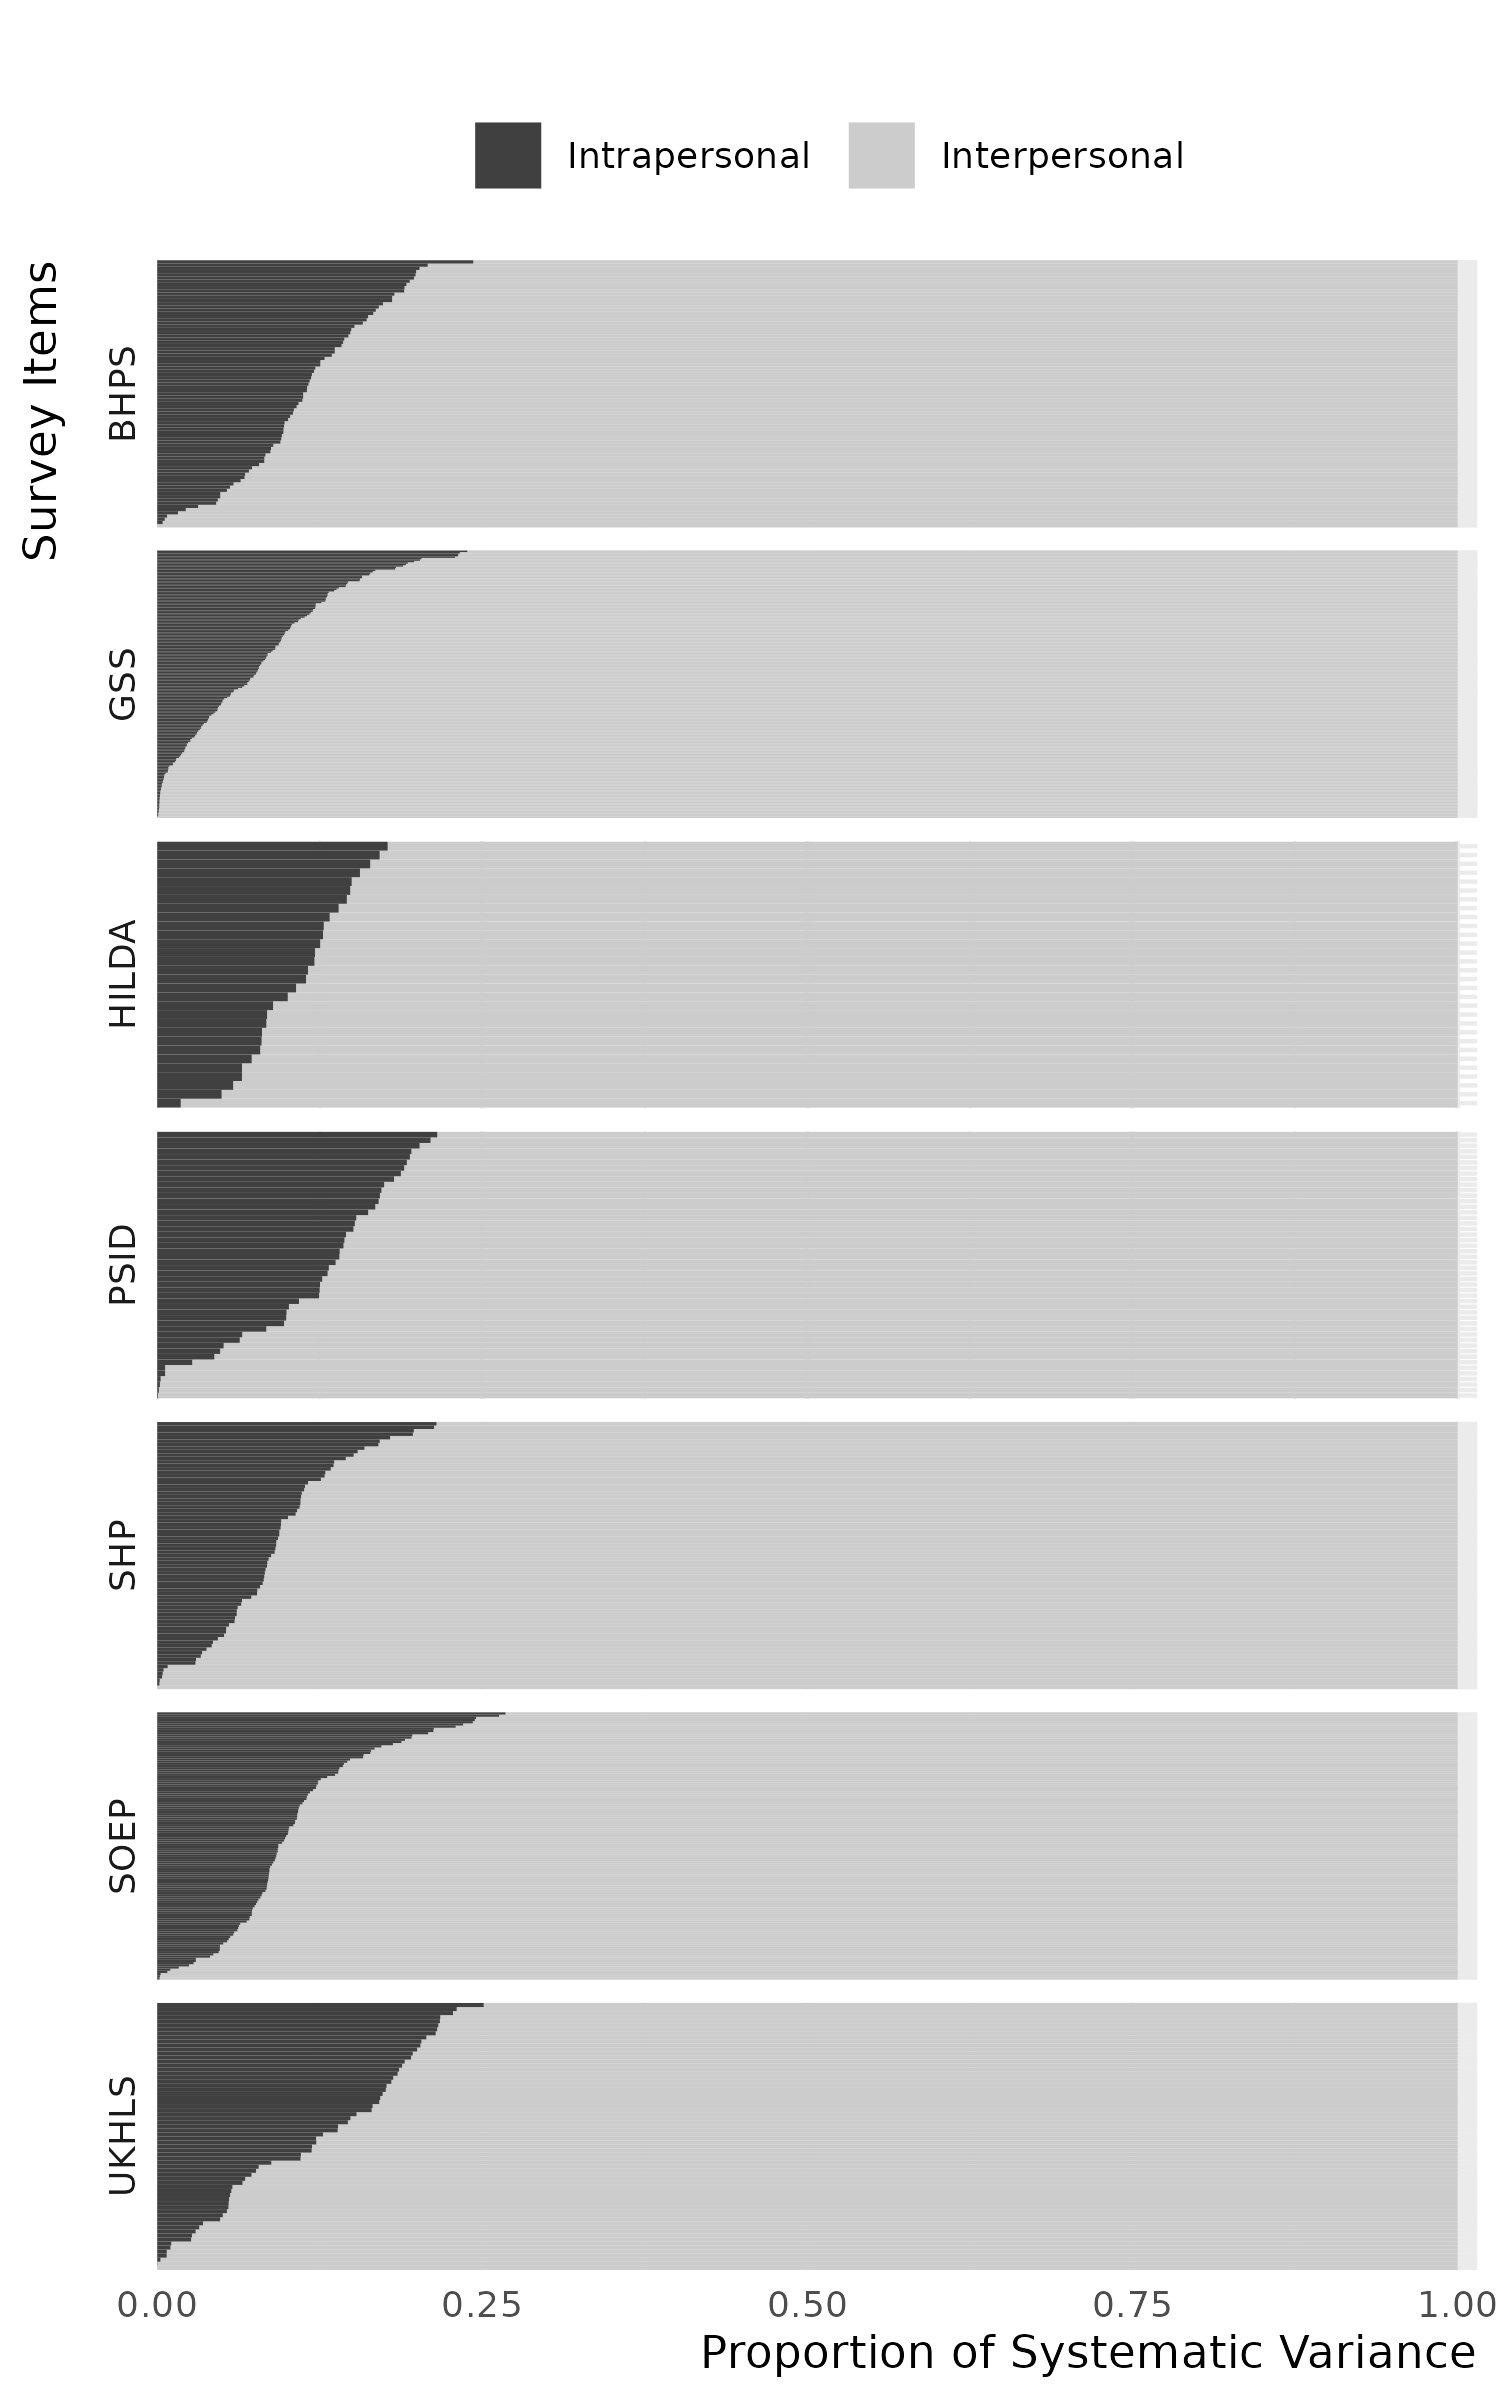
\includegraphics[width=20.83in]{../figures/figure_1_bw} \end{center}

\textit{Notes:} The figure shows $\omega$ and 1 - $\omega$ as the proportion of systematic variance attributable to intrapersonal change and interpersonal differences, respectively. See Supplemental Materials A for the full set of item values. 
\end{figure}

\newpage

\begin{figure}[ht]
\caption{Regression Model Estimating $\omega$}

\begin{center}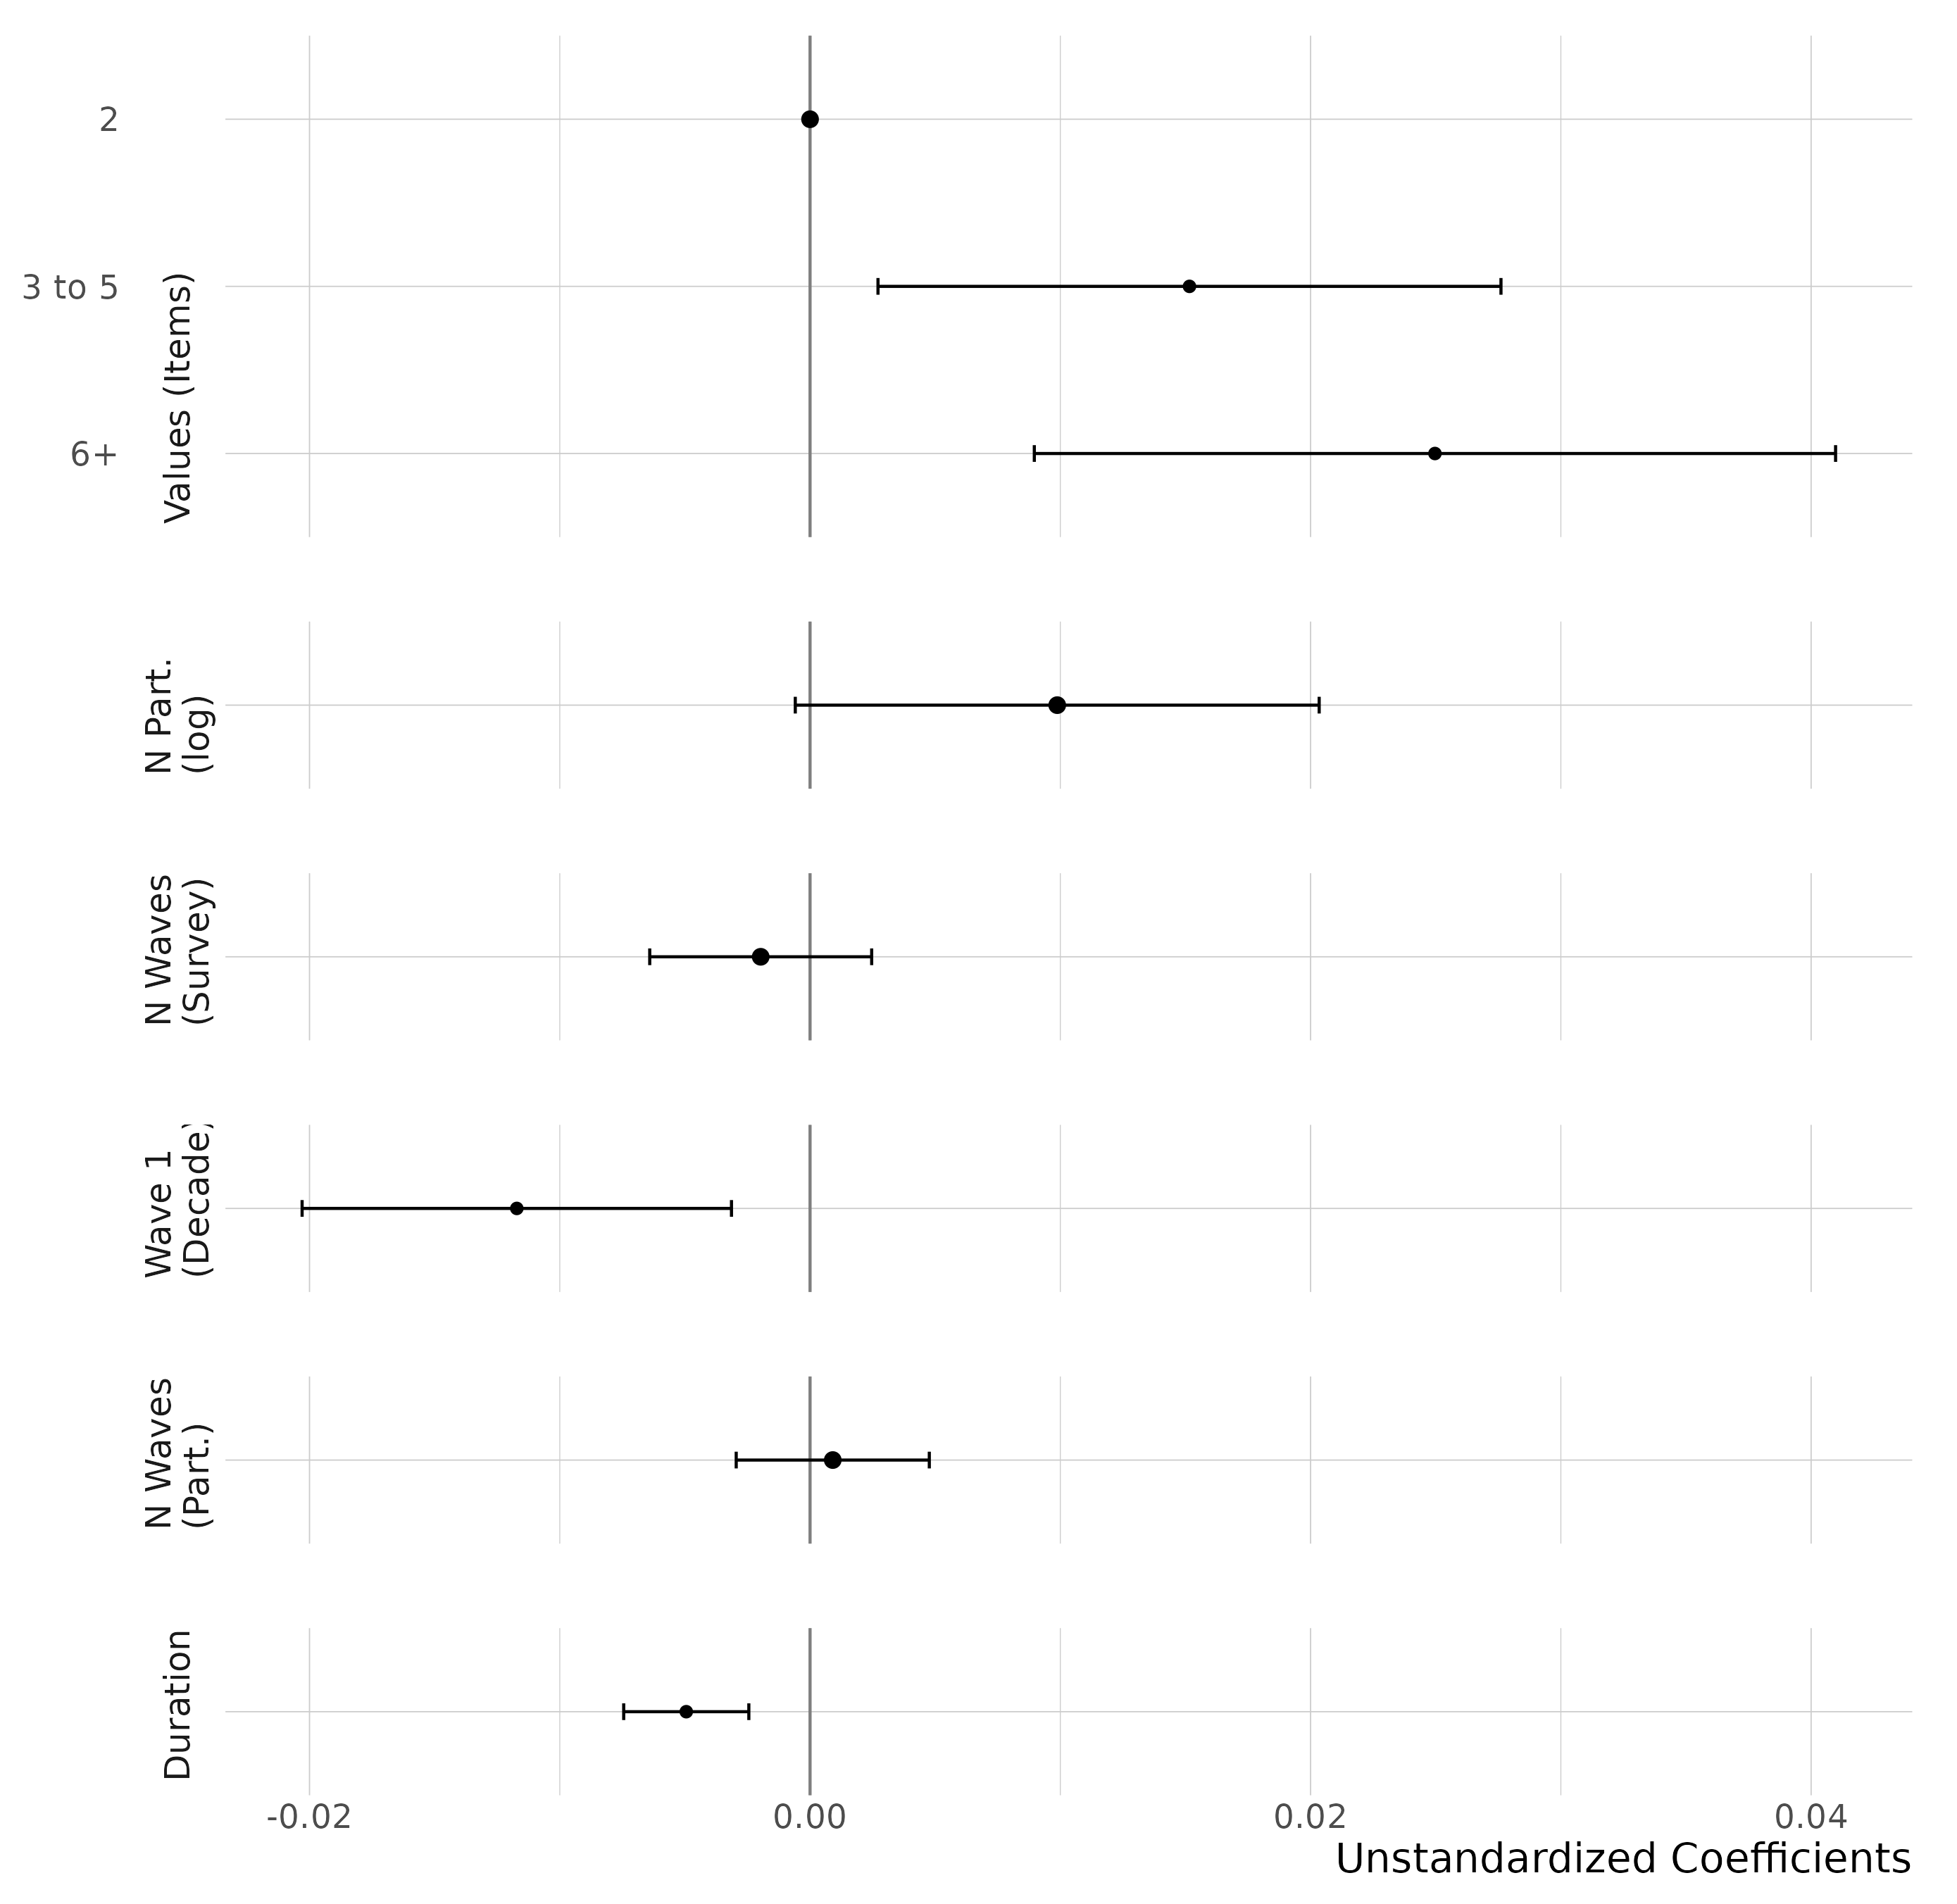
\includegraphics[width=300px]{../figures/figure_2} \end{center}

\textit{Notes:} The model estimates the proportion of systematic variance attributable to intrapersonal change. It includes the log of the number of participants, the number of waves the variable was asked (ceiled at t = 10 for each item), the date of the first wave (measured as the year minus 1968 divided by 10), number of waves the question was asked averaged across participants, duration in years per item averaged across participants, and panel and topic fixed effects. Coefficients are estimated from suppressed intercept model based on predictions at participants' wave mid-point. Survey indicators and item topics not shown. See Supplemental Materials B for the full set of coefficients.
\end{figure}

\newpage

\begin{figure}[ht]
\caption{Difference in $\omega$ Across College Graduates and Non-Graduates}

\begin{center}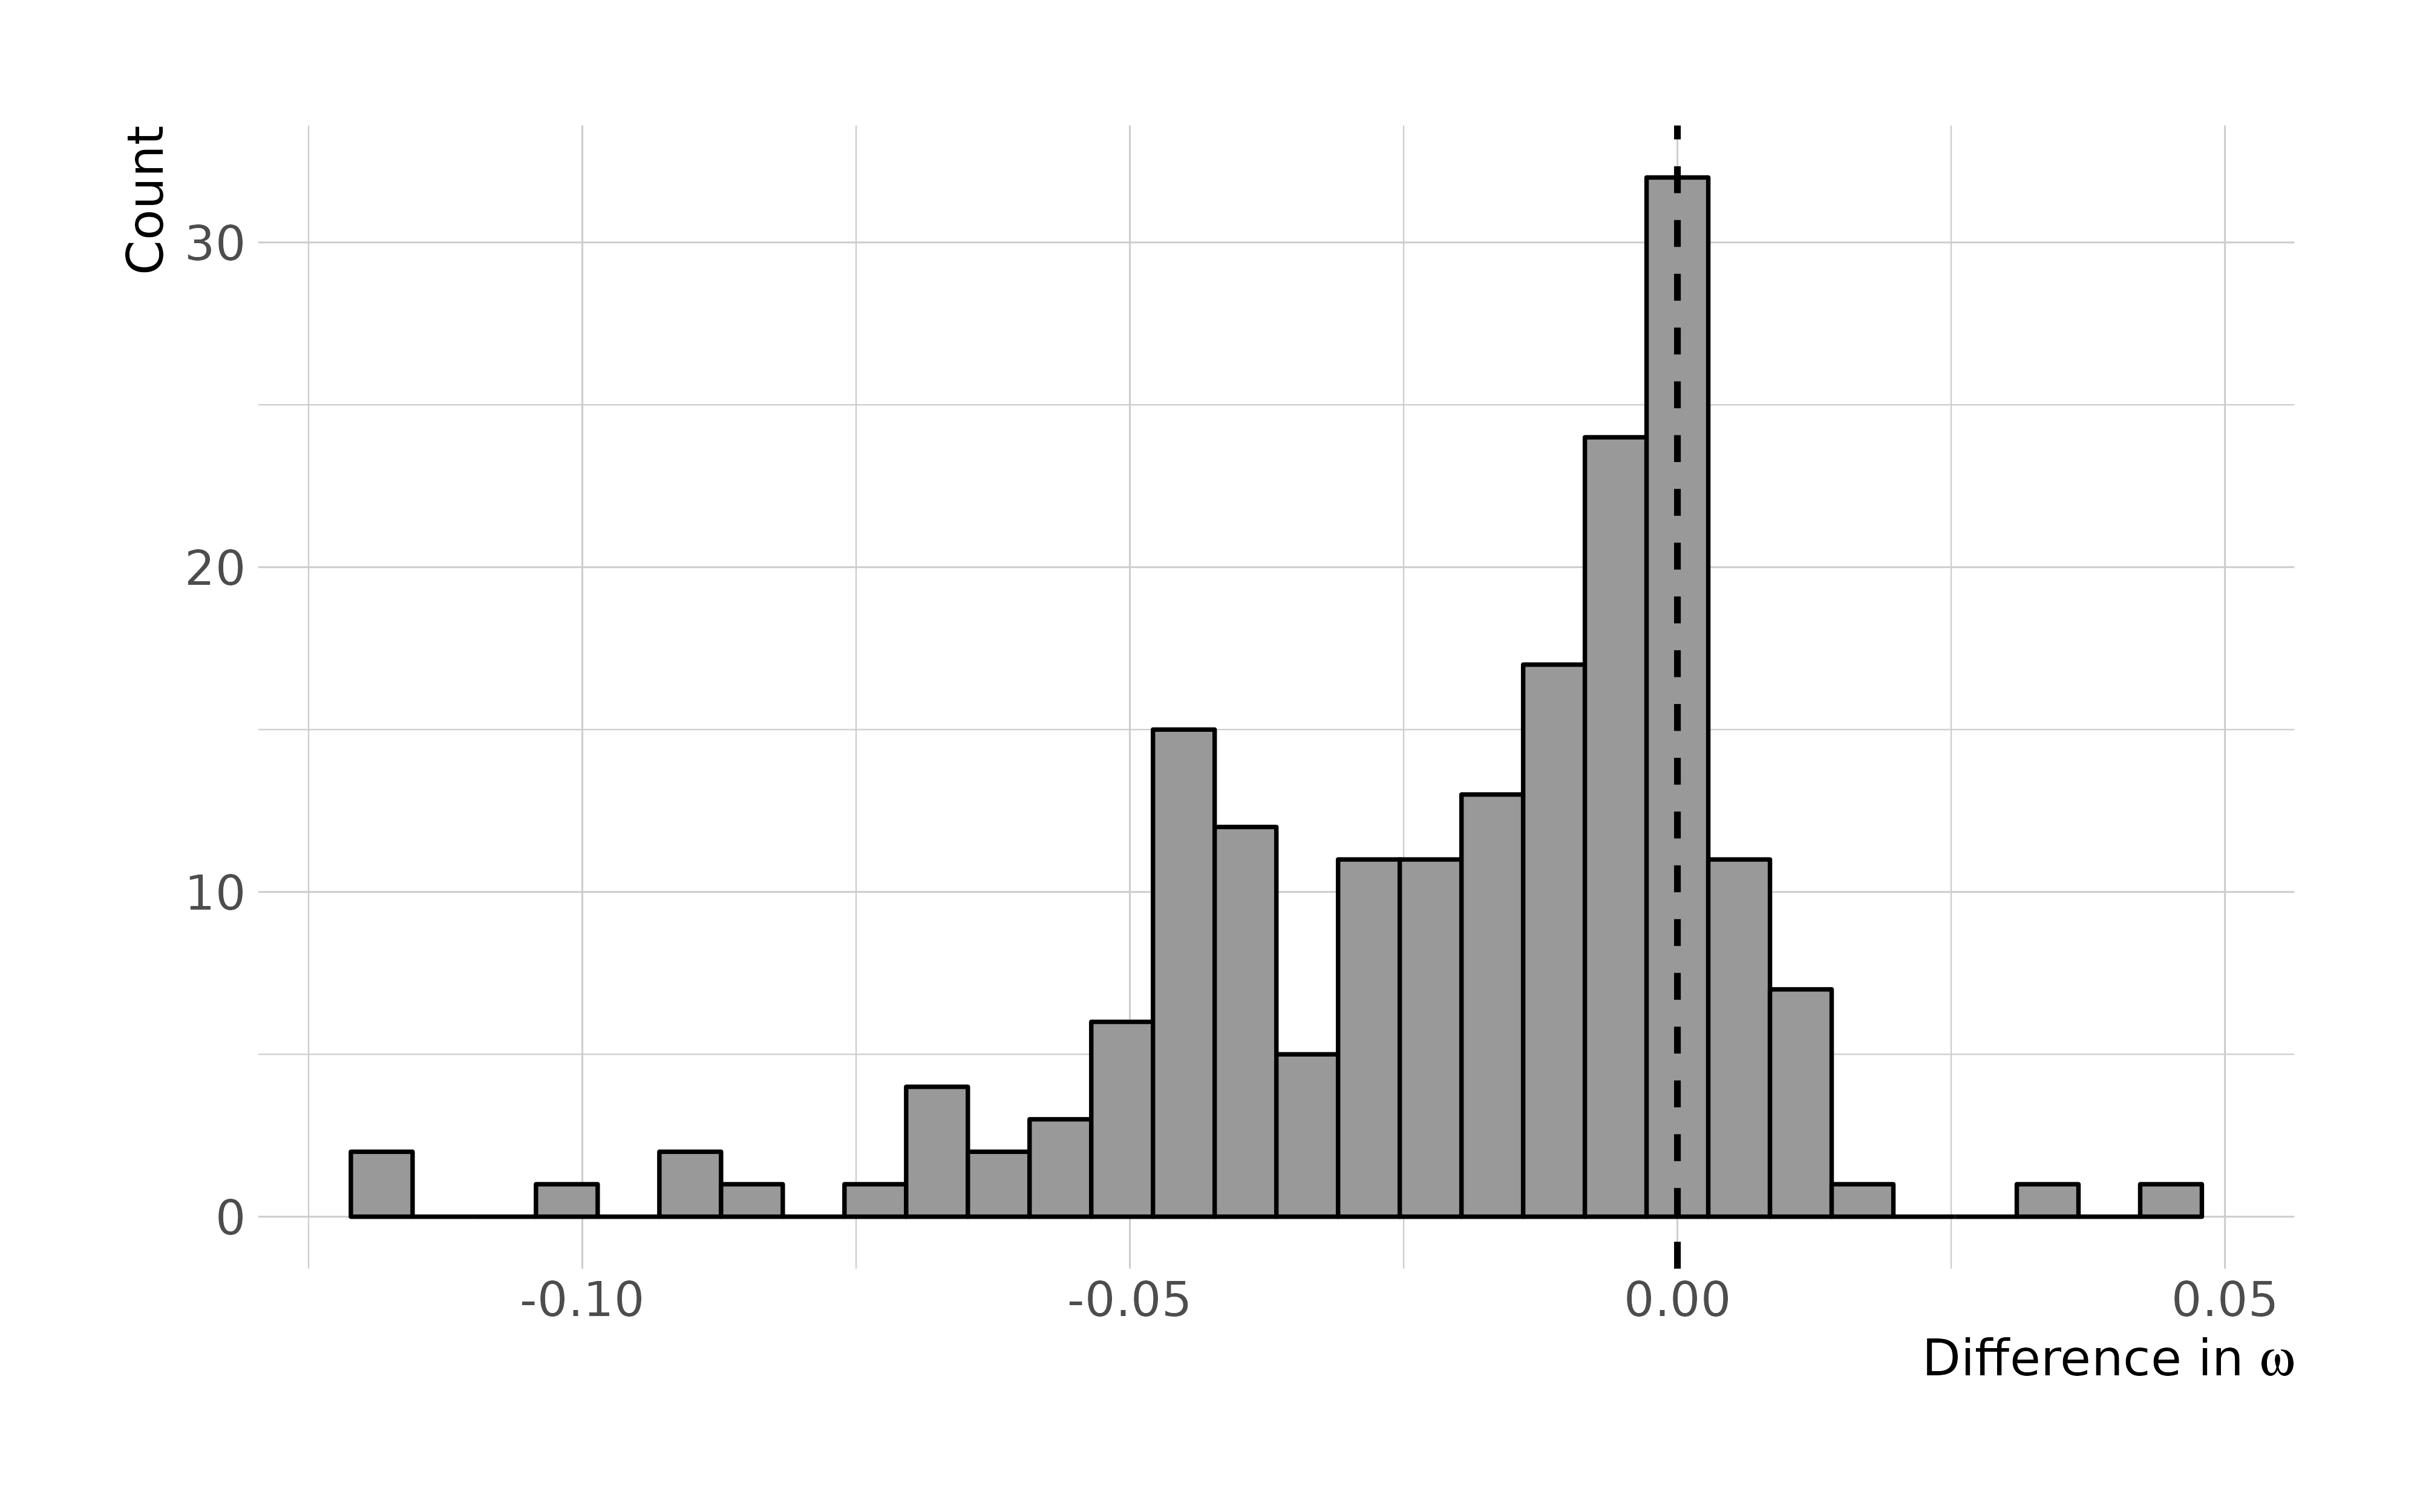
\includegraphics[width=450px]{../figures/figure_3_bw} \end{center}

\textit{Notes:} The figure shows the difference in $\omega$ values across college graduates and college non-graduates. Values above (below) 0 means that those with college degree have higher (lower) variance of intrapersonal change. The dashed red line marks 0 difference.
\end{figure}

\newpage

\begin{figure}[ht]
\caption{Difference in $\omega$ Across College Graduates and Non-Graduates on Political Culture}

\begin{center}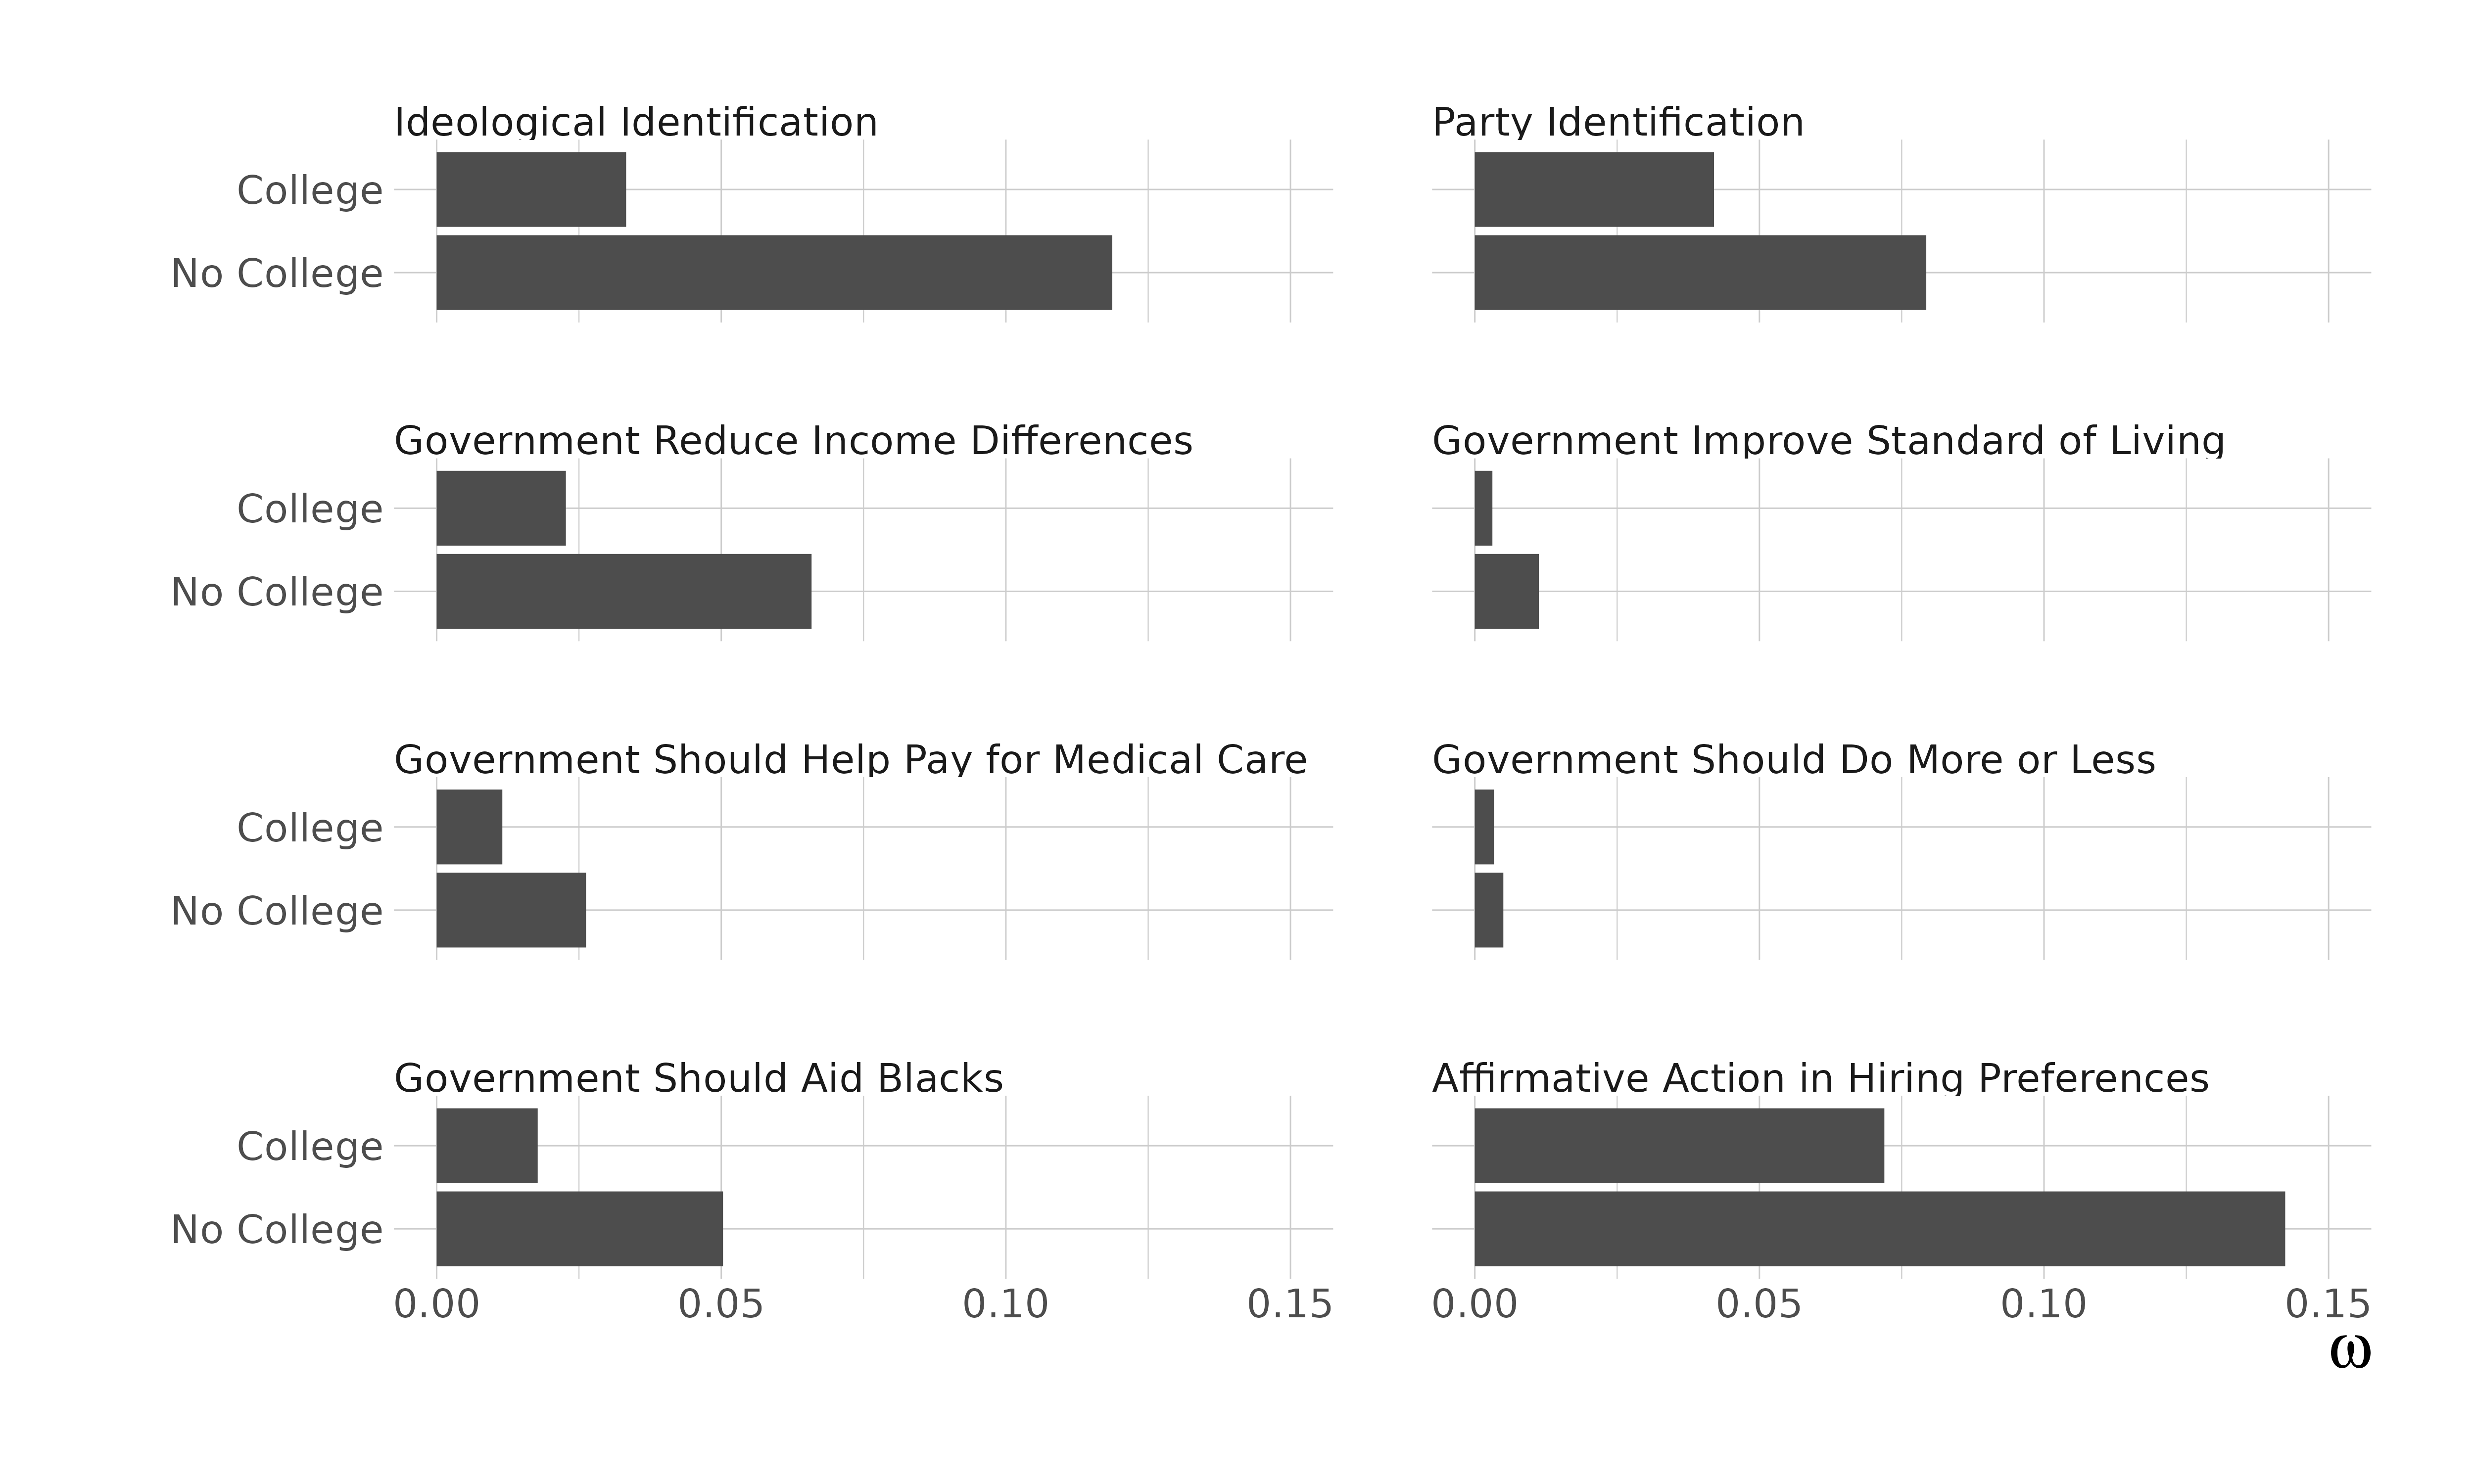
\includegraphics[width=450px]{../figures/figure_4_bw} \end{center}

\textit{Notes:} $\omega$ values across college graduates and college non-graduates on 8 political culture items from the General Social Survey (2006-2014).
\end{figure}

\end{document}
